\documentclass[12pt]{article}

% --- PREAMBLE ---
% --- XeLaTeX/Font setup ---
\usepackage{fontspec}           % 一定要最先加载
% \setmainfont{Latin Modern Roman}   % TeX Live 通常自带
\usepackage{appendix}
\usepackage{fourier-otf}        % OpenType 版 Fourier 数学字体

% --- 其余宏包 ---
\usepackage[english]{babel}     % 语言
\usepackage{graphicx}            % 插图
\usepackage{subcaption}
\usepackage{xcolor}              % 颜色
\usepackage{geometry}            % 版边
\usepackage[authoryear]{natbib}  % 文献引用
\usepackage{booktabs}            % 表格美化
\usepackage{tabularx}
\usepackage{amsthm}              % 定理环境···
\usepackage{setspace}
\usepackage{tikz}                % 图形绘制
\usepackage{hyperref}            % 超链接
\usetikzlibrary{positioning,calc,arrows.meta}
\onehalfspacing
% % 定理样式
% \theoremstyle{definition}
% \newtheorem{definition}{Definition}

% 页面设置
\geometry{a4paper, margin=1in}
\hypersetup{
  colorlinks,
  citecolor=blue,
}  % For better tables



% Define the "definition" environment style
\theoremstyle{plain}
\newtheorem{definition}{Definition}
\newtheorem{proposition}{Proposition}
\newtheorem{lemma}{Lemma}
\newtheorem{corollary}{Corollary}


% --- TITLE BLOCK ---
\title{Default with Pessimism}
\author{Chen Gao \thanks{National School of Development, Peking University. Email: \url{chengao0716@gmail.com}. I thank Bo Li and Changhua Yu for thorough guidance. I thank Michael Devereux for helpful advice.}}
\date{{\color{red} [INCOMPLETE AND PRELIMINARY]} \\ \today}

% --- DOCUMENT START ---
\begin{document}

\maketitle

\begin{abstract}
	Why do emerging economies face persistently high borrowing costs despite moderate debt levels? I develop a quantitative sovereign default model where lenders systematically overestimate government policy randomness. This behavioral bias creates a ``pessimism wedge'' that pivots bond prices---making debt cheaper near default but more expensive in normal times. Rational sovereigns respond by deleveraging yet paradoxically face higher average spreads and an ``illusion of financial stability'' where volatility falls despite higher risk premiums. Theoretical extensions demonstrate that optimal fiscal policy cannot eliminate allocative distortions from pessimism, negative learning bias perpetuates pessimistic beliefs, and strategic communication can partially mitigate these effects. The framework provides a new behavioral foundation for understanding sovereign debt puzzles in emerging markets.
\end{abstract}

\noindent \textbf{Keywords:} Sovereign Default, Behavioral Macroeconomics, Lender Pessimism, Sovereign Spreads, Information Frictions, Argentina, Debt Management.

\noindent \textbf{JEL Codes:} F34, E62, G15, D91.

\clearpage

\section{Introduction}
\label{sec:intro}

Why is sovereign debt in some emerging economies particularly expensive?
Standard models struggle to explain why countries with moderate debt-to-GDP
ratios face persistently high borrowing costs, excess volatility, and puzzling
``decoupling'' from their peers \citep{TomzWright2013,
	MeyerReinhartTrebesch2022}. Argentina exemplifies this puzzle: as documented by
\citep{MorelliMoretti2023}, its borrowing costs often appear divorced from
macroeconomic fundamentals, suggesting a large country-specific risk premium
that defies conventional explanation.

The leading explanation centers on reputation and \textit{information
	frictions} \citep{ColeDowEnglish1995}. In this view, advanced quantitatively by
\citep{MorelliMoretti2023}, lenders are rational but uninformed about a
government's hidden type---whether ``committed'' or ``strategic.'' Policy
missteps like Argentina's inflation misreporting signal a ``bad type,'' causing
persistent reputation downgrades. High spreads reflect the market's efficient
pricing of this revealed information.

This paper explores an alternative \textit{behavioral friction}. What if the
problem is not what lenders do not know, but what they systematically believe
to be true? Departing from rational learning, I posit that lenders suffer from
pessimistic bias about government policy randomness. While sovereigns face
unobserved ``taste shocks,'' lenders perceive these shocks as larger and more
volatile than they truly are. This ``pessimism wedge'' distorts default risk
assessment. Events like Argentina's misreporting signal not just strategic
behavior but perceived policy unpredictability. Markets react to this perceived
randomness increase beyond mere reputation downgrades.

My main contribution embeds this behavioral friction into a quantitative
sovereign default model and traces its macroeconomic consequences. Pessimistic
lenders fundamentally alter the borrowing environment by ``pivoting'' bond
price schedules---making debt cheaper near default but more expensive in safe
states. Rational sovereigns respond optimally by deleveraging yet paradoxically
face higher average spreads. The model generates an ``illusion of financial
stability'' where market volatility falls despite rising risk premiums.

Three theoretical extensions deepen the analysis. First, even optimal Ramsey
fiscal policy cannot eliminate welfare losses from pessimism due to fundamental
allocative inefficiencies from distorted bond pricing. Second, endogenous
belief formation through Bayesian learning with negativity bias shows how
pessimistic beliefs persist and become entrenched. Third, optimal policy
communication demonstrates how governments can strategically choose
transparency levels to partially mitigate lender pessimism. The analysis
provides a new behavioral foundation for understanding sovereign risk and
persistent debt challenges in emerging economies.

\paragraph{Literature} This paper contributes to the sovereign default literature by proposing a novel
behavioral mechanism to explain persistent empirical puzzles: why do emerging
economies often face high spreads and excess volatility that seem disconnected
from their macroeconomic fundamentals \citep{TomzWright2013,
	MitchenerTrebesch2023}?\footnote{For comprehensive surveys of the sovereign
	debt literature, see \citep{MeyerReinhartTrebesch2022} and \citep{Abbas2019}.}

The dominant paradigm treats default as a purely \textit{strategic decision}
where sovereigns rationally weigh repayment costs against temporary market
exclusion \citep{EatonGersovitz1981, AguiarGopinath2007, Arellano2008}. While
this framework has been successfully extended to incorporate long-term debt and
financial frictions \citep{HatchondoMartinez2009, ChatterjeeEyigungor2012,
	MendozaYue2012},\footnote{Empirical evidence on emerging market business cycles
	and debt restructurings is provided by \citep{NeumeyerPerri2005},
	\citep{CrucesTrebesch2013}, and \citep{ArellanoRamanarayanan2012}.} it
struggles to explain why spreads often remain elevated even when fundamentals
improve.

A second approach emphasizes \textit{reputational concerns}, where past actions
cast long shadows over future borrowing costs \citep{ColeDowEnglish1995,
	Phelan2006}. In this framework, the central question is how lenders learn about
the government's hidden type. While classic models focus on default itself as
the ultimate signal, recent research shows the informational channel is much
broader. For instance, \citep{Fourakis2021} provides quantitative evidence that
investors learn about government types through fiscal and monetary policy
indicators, finding that deficit and inflation surprises significantly affect
perceived default probabilities and that reputation loss often occurs
\textit{before} a default event. This perspective is powerfully exemplified by
the Argentina inflation misreporting episode, rigorously analyzed by
\citep{MorelliMoretti2023}, where a single breach of trust—interpreted as a
credible signal of a ``bad type''—led to years of market exclusion.This rich
view of reputation has been embedded in models that explain how a country can
eventually "graduate" to a high-trust state through a long history of good
behavior \citep{AmadorPhelan2021} and why, in a partial default setting, larger
haircuts must rationally lead to a greater loss of reputation to sustain a
mixed-strategy equilibrium \citep{AmadorPhelan2023}.\footnote{Other important
	contributions to the reputation literature include \citep{ColeKehoe1998} on
	partial versus general reputations, \citep{DErasmo2011} on government
	reputation and debt repayment, \citep{EgorovFabinger2016} on reputational
	effects in sovereign default, and \citep{DovisKirpalani2020,
		DovisKirpalani2021} on reputation in policy design. A key distinction is that
	while reputation models predict "bad types" default at lower debt thresholds,
	my pessimism model counterintuitively predicts the opposite: pessimistic
	lenders perceive higher default thresholds due to overestimated policy
	randomness.} Yet even this learning-based view assumes lenders eventually
converge to the truth, leaving unexplained why some sovereign risk premia
appear systematically and persistently excessive.

A third strand recognizes that market \textit{sentiment itself} can become a
fundamental force. Beginning with \citep{CalvoLeidermanReinhart1996} and
\citep{ColeKehoe2000}, this literature demonstrates how pessimistic
expectations can become self-fulfilling, with modern quantitative
implementations by \citep{GennaioliMartinRossi2014} and
\citep{BocolaDovis2019}.\footnote{Related work explores financial frictions
	\citep{LongstaffPanPedersenSingleton2011}, risk aversion \citep{Lizarazo2013},
	maturity choice \citep{Stangebye2020}, and rational learning about shifts in
	fundamentals, such as the "rare disaster" mechanism in \citep{Paluszynski2023}
	used to explain the slow onset of the European debt crisis.} My paper builds
directly on this insight but asks a deeper question: what if markets
systematically \emph{misperceive} the very nature of sovereign decision-making?

Drawing from behavioral economics, I propose that lender pessimism---rooted in
well-documented biases like \textit{heuristics and biases}
\citep{TverskyKahneman1974}, \textit{prospect theory}
\citep{KahnemanTversky1979}, and \textit{noise trading}
\citep{DeLongEtAl1990}---can create persistent wedges between sovereign risk
and fundamentals.\footnote{Additional behavioral foundations include investor
	sentiment \citep{BakerWurgler2006}, rare disasters \citep{Gabaix2012},
	disposition effects \citep{ShefrinStatman1985}, crisis psychology
	\citep{Kindleberger1978}, and limits to arbitrage \citep{BrunnermeierNagel2004,
		BarberisThaler2003}.} Crucially, my mechanism differs from existing behavioral
approaches. For instance, models of \textit{ambiguity aversion} based on robust
control theory \citep{GilboaSchmeidler1989, HansenSargent2008} assume that
lenders are uncertain about the true model of macroeconomic fundamentals. This
leads them to price assets based on a "worst-case" scenario, generating an
ambiguity premium that can explain high sovereign spreads
\citep{PouzoPresno2016} and the puzzlingly poor pricing of contingent debt
\citep{RochRoldan2023}. While these models distort the perceived distribution
of \textit{macroeconomic shocks} across all states, my ``pessimism wedge''
specifically targets the perceived volatility of the sovereign's \textit{policy
	choices}, creating a distinctive bond-price \textit{pivot}.\footnote{This pivot
	effect contrasts sharply with both reputation and ambiguity aversion models.
	While reputation models like \citep{AmadorPhelan2021} generate monotonic price
	effects through type revelation and \citep{Fourakis2021} shows reputation loss
	\textit{before} default through rapid debt accumulation, my model produces
	non-monotonic price schedules where debt becomes cheaper near default but more
	expensive in normal times. Similarly, ambiguity models like
	\citep{RochRoldan2023} explain high spreads through a uniform distortion of
	fundamental shocks, which also differs from the pivot mechanism.} And unlike
\textit{diagnostic expectations} \citep{GennaioliShleifer2018,
	BordaloEtAl2023}, which generate boom-bust cycles through time-varying news
overreaction, my time-invariant bias produces persistent ``pessimism premia,''
counterintuitive deleveraging, and the ``softening-of-doom'' effects that
standard models cannot replicate.\footnote{The empirical predictions also
	differ markedly from reputation models. While \citep{MorelliMoretti2023} find
	that misreporting episodes increase spreads on all debt instruments, my model
	predicts divergent effects across the debt distribution. Similarly, while
	\citep{AmadorPhelan2023} shows reputation effects strengthen with haircut size,
	my pessimism model predicts that pessimism effects would weaken as larger
	haircuts reduce the perceived randomness component.}

% --- MOTIVATION ---------------------------------------------------------------
\section{Motivation: Argentina's Inflation--Misreporting Episode}
\label{sec:motivation}

\paragraph{A Puzzle of Persistent Risk}
The recent economic history of Argentina offers a powerful illustration of a
core puzzle in international finance: why do emerging economies often face
borrowing costs that seem disconnected from their macroeconomic fundamentals?
\citep{TomzWright2013, MeyerReinhartTrebesch2022}. Standard models, even those
incorporating reputational dynamics, struggle to fully account for the
persistence and magnitude of the country-specific risk premium observed in
cases like Argentina, where borrowing costs have often appeared divorced from
traditional measures of repayment capacity \citep{MorelliMoretti2023}. This
suggests the presence of frictions beyond those typically modeled.
	{\color{red}[TODO: Add comparison table showing Argentina vs Brazil/Chile core
			indicators (debt ratio, GDP growth, spreads) to more intuitively highlight the
			``anomaly'' mentioned in reviewer feedback]}

\paragraph{The Misreporting Episode}
This puzzle was cast in sharp relief during the inflation misreporting episode
that began in 2007. Following a period of rising inflation, the Argentine
government initiated a direct political intervention in its national statistics
institute, INDEC. Senior technical staff were dismissed and replaced, leading
to an immediate and sustained suppression of the official Consumer Price Index
(CPI) \citep{MorelliMoretti2023}. This official figure diverged starkly from
credible estimates produced by private and provincial sources
\citep{Cavallo2013}. The government's enforcement was aggressive, levying
substantial fines on private consultancies that published their own, more
realistic, data \citep{ReutersFines2013}. The data manipulation grew so
notorious that \textit{The Economist} publicly ceased publishing the official
figures in 2012, and the IMF issued a rare ``declaration of censure'' against
the country \citep{Economist2012, IMFPress2013}.

The financial consequences were profound. As inflation-indexed bonds
constituted a significant portion of public debt, this act amounted to a
\textit{de facto} partial default. The market's reaction was swift and severe.
Argentina's EMBI+ spread, which had been tracking its Latin American peers,
decoupled and widened sharply. Crucially, this repricing was not limited to the
directly affected instruments; it spilled over entirely to its
dollar-denominated sovereign debt. This reaction is paradoxical from a purely
mechanical standpoint: a policy that lowers the real debt burden should have
\textit{decreased} default risk on nominal bonds. The opposite happened,
indicating the event was a pure, and powerful, information shock about the
government's character and future actions.

	% \begin{figure}[htbp]
	% 	\centering
	% 	{\color{red}[TODO: Download the new data from a Bloomberg terminal and save it in the Empirics folder]}
	% 
	% 	\includegraphics[width=0.6\textwidth]{../../long_term/Empirics/Results/Figure_EMBI_LATAM.pdf}
	% 	\caption{Argentina's EMBI+ spread relative to the Latin-American average,
	% 		2006–2012.  The shaded area marks the period starting in 2007 when INDEC's CPI
	% 		methodology was politically controlled.
	% 		Source:~J.~P.~Morgan.}
	% 	\label{fig:argentina_spreads}
	% \end{figure}

	[Figure placeholder: Argentina's EMBI+ spread data - TODO: Download from Bloomberg terminal]

\paragraph{Limits of Reputational Models}
The conventional explanation, rooted in reputational models
\citep{ColeDowEnglish1995}, interprets this episode as a credible signal of a
"bad type." In this view, advanced by \citep{MorelliMoretti2023}, lenders are
rational but uninformed about a government's hidden commitment to repay. The
misreporting revealed Argentina's government as a ``strategic'' type, leading
to a rational, persistent downgrade of its reputation and, consequently, higher
borrowing costs. While this view is powerful, it leaves lingering questions. If
the market simply learned the government's type, why did the risk premium
appear to contain an additional, seemingly excessive, component? Why did market
sentiment seem to reflect not just a reassessment of character, but a new
apprehension about the government's very predictability? The episode suggests
that the market's reaction was not just to what it learned about the
sovereign's \textit{intent}, but to a perceived increase in its \textit{erratic
	nature}.

\paragraph{A Behavioral Hypothesis: Lender Pessimism}
This paper explores an alternative, yet complementary, behavioral friction. I
posit that the problem is not only what lenders do not know, but also what they
systematically, and pessimistically, believe to be true. My core assumption is
that lenders perceive the unobserved shocks driving sovereign policy choices to
be larger and more volatile than they truly are. This ``pessimism wedge''
distorts their assessment of default risk. From this perspective, an event like
Argentina's misreporting is not just a signal of a sovereign's bad character (a
strategic type), but is interpreted as evidence of its erratic nature (high
unpredictability). The market reacts to a perceived increase in policy
randomness, not just a downgrade of its reputation. This pessimism is not
irrational in a colloquial sense; rather, it is a systematic bias in belief
formation, consistent with behavioral findings on how agents process
information under uncertainty \citep{TverskyKahneman1974, BarberisThaler2003}.

\paragraph{A Bridge to the Model}
Motivated by this reinterpretation of the Argentine case, I embed this
behavioral friction into an otherwise standard quantitative sovereign default
model. The subsequent sections will formalize the ``pessimism wedge'' and trace
its consequences. I will show that the presence of pessimistic lenders
fundamentally alters the sovereign's borrowing environment, creating a
distinctive "pivoting" of the bond price schedule. This, in turn, generates a
series of counterintuitive but empirically relevant outcomes: a rational
sovereign deleverages yet faces higher average spreads, and market volatility
can fall even as the underlying risk premium rises, creating an ``illusion of
financial stability.'' This framework provides a new, behaviorally-grounded
perspective on the persistent debt challenges that many emerging economies
face.

\section{A Model of Pessimism}
\label{sec:model}

\subsection{Environment}
Time is discrete and the horizon is infinite, $t = 0, 1, 2, \dots$. The economy
receives a stochastic endowment of a single tradable good, $y_t$. The endowment
process is exogenous and follows a stationary, first-order Markov process,
which is generated by discretizing the following AR(1) process in logarithms:
\begin{equation}
	\ln y' = (1-\rho_y)\mu_y + \rho_y \ln y + \sigma_y \varepsilon', \quad \varepsilon' \sim \mathcal{N}(0, 1).
	\label{eq:endowment}
\end{equation}
The transition probabilities are given by the matrix $\Pi(y, y') = \Pr\{y_{t+1}=y'|y_t=y\}$.

The government can borrow from a large number of competitive, risk-neutral
international lenders who have access to an international risk-free interest
rate $r$. Debt takes the form of long-term bonds. A bond is a claim to a stream
of coupon payments $\kappa$ in every future period, unless the sovereign
defaults. Each period, a fraction $\delta \in (0, 1]$ of outstanding bonds
matures, while the remaining fraction $1-\delta$ carries over to the next
period.

The sovereign government has preferences represented by a standard
time-separable utility function with a discount factor $\beta \in (0, 1)$. The
period utility function is of the CRRA form:
\begin{equation}
	u(c) = \frac{c^{1-\sigma}-1}{1-\sigma},
\end{equation}
which is strictly increasing and concave for $\sigma > 0$.

\subsection{The Sovereign's Problem}
At the beginning of each period $t$, the state is summarized by the current
endowment realization $y \in \mathcal{Y}$ and the stock of outstanding debt
$B$. The sovereign first decides whether to default on its obligations or to
repay. This choice is subject to an idiosyncratic preference shock, often
referred to as a ``taste shock,'' which introduces randomness into the
decision-making process from the perspective of an outside observer.

\paragraph{Taste Shocks}
Let $V^D(y)$ be the deterministic component of the value of defaulting, and
$V^R(y, B)$ be the deterministic component of the value of repaying. The full,
or \textit{ex-post}, value for each choice is the sum of its deterministic part
and a random shock:
\begin{align*}
	\tilde{V}^D(y, \varepsilon_d)    & = V^D(y) + \varepsilon_d    \\
	\tilde{V}^R(y, B, \varepsilon_r) & = V^R(y, B) + \varepsilon_r
\end{align*}
The sovereign observes the shocks $\varepsilon_d$ and $\varepsilon_r$ and chooses the action that yields the highest \textit{ex-post} value. The \textit{ex-ante} value function, from a perspective before the shocks are realized, is the expected maximum of these \textit{ex-post} values:
\begin{equation}
	V(y, B) = \mathbb{E}_{\varepsilon_d, \varepsilon_r} \left[ \max \left\{ \underbrace{V^D(y) + \varepsilon_d}_{\tilde{V}^D(y, \varepsilon_d)}, \underbrace{V^R(y, B) + \varepsilon_r}_{\tilde{V}^R(y, B, \varepsilon_r)} \right\} \right],
\end{equation}
where the expectation is taken over the distribution of the shocks.

Following \citep{DvorkinSancheSaprizaYurdagul2021} and
\citep{MIHALACHEOREEF2024}, I assume that the taste shocks $\varepsilon_d$ and
$\varepsilon_r$ are drawn independently from a Gumbel
distribution.\footnote{The CDF of a Gumbel distribution is given by
	$F(\varepsilon; \mu_L, \eta) = \exp(-\exp(-(\varepsilon-\mu_L)/\eta))$, where
	$\mu_L$ is the location parameter and $\eta > 0$ is the scale parameter. The
	mean of this distribution is $\mu_L + \eta\gamma$, where $\gamma \approx
		0.5772$ is the Euler-Mascheroni constant. For analytical convenience, I choose
	a specific parameterization, Gumbel$(-\eta\gamma, \eta)$, which makes the mean
	of the shocks equal to zero: $\mathbb{E}[\varepsilon_i] = -\eta\gamma +
		\eta\gamma = 0$.} To visualize the distribution of these shocks,
Figure~\ref{fig:gumbel_dist} plots the probability density function (PDF) and
cumulative distribution function (CDF) for the Gumbel distribution, normalized
to have a mean of zero. The scale parameter, $\eta$, is pivotal. It governs the
variance of the taste shocks, given by $\text{Var}(\varepsilon_i) = \frac{\pi^2
		\eta^2}{6}$. A larger $\eta$ signifies greater dispersion in preferences and
introduces more randomness into the sovereign's choice.\footnote{As $\eta \to
		0$, the shocks' influence diminishes, and the model approaches a deterministic
	framework where decisions are based solely on $V^D(y)$ and $V^R(y,B)$.
	Conversely, as $\eta \to \infty$, the deterministic value components become
	negligible, and the choice becomes almost entirely random.} Economically, these
taste shocks can be interpreted as a reduced-form representation of various
unmodeled factors that influence policy, such as political pressures from
domestic constituencies, bureaucratic implementation errors, or the private
information of policymakers. By modeling them as random draws, the framework
acknowledges a degree of inherent unpredictability in government behavior.
\begin{figure}[htbp]
	\centering
	\includegraphics[width=0.6\textwidth]{gumbel_distribution.png}
	\caption{The mean-zero Gumbel distribution ($\eta=5\times 10^{-4}$).}
	\label{fig:gumbel_dist}
	\parbox{\linewidth}{\small\textit{Note:} The Gumbel distribution is used to model the taste shocks in the sovereign's default and borrowing decisions. The scale parameter $\eta$ controls the variance of these shocks. The left $y$ axis is the PDF, the right $y$ axis is the CDF.}
\end{figure}

\paragraph{Ex-Ante Value Function}
The ex-ante value function can be derived using fundamental properties of the
Gumbel distribution. The lemma provided in Appendix \ref{app:gumbel} provides
the closed-form expression for the expected maximum of Gumbel-distributed
random variables, which forms the basis for my analytical solution. First,
applying Lemma~\ref{lem:gumbel_max_expectation} to my setting with $V_1 =
	V^D(y)$ and $V_2 = V^R(y, B)$, the ex-ante value function is:
\begin{equation}\label{eq:V_choice}
	V(y, B) = \mathbb{E}\left[\max\{\tilde{V}^d, \tilde{V}^r\}\right] = \eta \ln\left( \exp\frac{V^D(y)}{\eta} + \exp\frac{V^R(y, B)}{\eta} \right).
\end{equation}

\paragraph{Discrete Choice}
The choice probabilities in my model follow directly from another fundamental
property of the Gumbel distribution. Using Lemma~\ref{lem:gumbel_logit} in
Appendix \ref{app:gumbel}, the probability of default is:
\begin{equation}\label{eq:prd_1}
	\Pr\{d=1 | y, B\} = \frac{\exp\frac{V^D(y)}{\eta}}{\exp\frac{V^D(y)}{\eta} + \exp\frac{V^R(y, B)}{\eta}}.
\end{equation}

\paragraph{Value of Default}
If the sovereign defaults, it is excluded from international credit markets.
During exclusion, it bears an output cost and consumes a fraction of its
endowment, $c = h(y) \le y$, where the output cost function is specified
similar to \citep{ChatterjeeEyigungor2012}:
\begin{equation}
	h(y) = y - \max\{0, \lambda_0 y + \lambda_1 y^2\}.
\end{equation}
In each period of exclusion, there is a constant probability $\gamma \in (0, 1)$ that the country regains market access. Upon re-entry, all past debts are forgiven, so it starts with $B=0$. The value of being in default is therefore:
\begin{equation}
	V^D(y) = u(h(y)) + \beta \mathbb{E}_{y'|y} \left[ \gamma V(y', 0) + (1-\gamma) V^D(y') \right].
	\label{eq:Vd}
\end{equation}

\paragraph{Value of Repayment }
If the sovereign honors its debt, it pays the coupon $\kappa B$ and retains
market access. It can then choose a new level of debt for the next period,
$B'$. This choice is also subject to taste shocks. The \emph{ex-ante} value of
choosing a specific debt level $B'$, given the state $(y, B)$, is:
\begin{equation}
	W(y, B, B') = u\left(y - \kappa B + \left[B' - (1-\delta)B\right] q(y, B')\right) + \beta \mathbb{E}_{y'|y} \left[V(y', B')\right],
\end{equation}
where $q(y, B')$ is the price at which it can issue new bonds. The borrowing choice is subject to i.i.d. Gumbel shocks, denoted by
$\{\varepsilon_{B'}\}$, for each possible debt level $B'$. Each shock is
distributed as Gumbel$(-\rho\gamma, \rho)$. Applying Lemma~\ref{lem:gumbel_multinomial} in Appendix \ref{app:gumbel} with $V_i = W(y, B, B_i)$ and
$\sigma = \rho$, the ex-ante value of repaying is:
\begin{equation}\label{eq:Vr}
	V^R(y, B) = \rho \ln\left( \sum_{B' \in \mathcal{B}} \exp\frac{W(y, B, B')}{\rho} \right),
\end{equation}
where $\mathcal{B}$ is the discrete set of possible debt levels. The probability of choosing a specific level $B'$ is:
\begin{equation}
	\Pr\{B' | y, B\} = \frac{\exp\frac{W(y, B, B')}{\rho}}{\sum_{B_j \in \mathcal{B}}\exp\frac{W(y, B, B_j)}{\rho}}.
\end{equation}
ssFigure~\ref{fig:borrowing_dist_example} provides a visualization of this
probabilistic borrowing policy. The taste shock framework transforms the choice
of the next debt level, $B'$, from a single deterministic point into a smooth
probability distribution over the entire set of available options,
$\mathcal{B}$. The peak of the distribution corresponds to the most preferred
borrowing choice, but the scale parameter $\rho$ ensures that other, less
optimal choices still have a non-zero probability of being selected. This
feature captures \textit{unobserved heterogeneity} in the sovereign's
decision-making process.\footnote{This probabilistic approach is also crucial
	for the numerical stability of the model, as it replaces the non-differentiable
	``max'' operator with a smooth, analytical expression, which is similar to the idea of \citep{ChatterjeeEyigungor2012}.}

\begin{figure}[h!]
	\centering
	\includegraphics[width=0.6\textwidth]{../../pessimism-default-model/results/comparison_figure_8.pdf}
	\caption{Example of the Probabilistic Borrowing Policy, $\Pr\{B'|y,B\}$.}
	\label{fig:borrowing_dist_example}
	\parbox{\textwidth}{\small\textit{\textbf{Note:} }The figure illustrates the sovereign's borrowing choice as a probability distribution over possible next-period debt levels ($B'$), given a specific state $(y, B)$. The peak of the distribution represents the most likely choice.}
\end{figure}

\subsection{International Lenders and Bond Pricing}

I depart from the standard model by assuming a \textit{wedge} between the
sovereign's true behavior and lenders' perception of it. Lenders in this model
are competitive and risk-neutral, pricing bonds to make zero expected profit
according to their beliefs. However, their beliefs are systematically biased in
a specific way.

\paragraph{Pessimism}The key assumption is that lenders perceive the sovereign to be more erratic or
``irrational'' than it truly is. They believe the sovereign's default decision
is governed by a taste shock with a scale parameter $\tilde{\eta} = \theta
	\cdot \eta$, where $\theta \ge 1$. The parameter $\theta$ captures the degree
of \textit{lender pessimism, parameter uncertainty, or ambiguity aversion.
}When $\theta > 1$, lenders act \textit{as if} the government's choices are
more random than they actually are.

Consequently, the lenders' perceived probability of default at a future state
$(y', B')$, which I denote $\tilde{P}(y', B')$, is calculated using this
inflated shock parameter similar to \eqref{eq:prd_1}:
\begin{equation}
	\tilde{P}(y', B') = \frac{\exp\frac{V^D(y')}{\theta\eta}}{\exp\frac{V^D(y')}{\theta\eta}+\exp\frac{V^R(y',B')}{\theta\eta}}.
	\label{eq:plender}
\end{equation}

\paragraph{Bond Price}The equilibrium bond price $q(y, B')$ must satisfy the no-arbitrage condition
based on these pessimistic beliefs. The price equals the discounted expected
payoff, where the probability of repayment is assessed using $\tilde{P}(y',
	B')$:
\begin{equation}
	\begin{aligned}
		q(y, B') & = \frac{1}{1+r} \mathbb{E}_{y'|y} \left[ \left(1 - \tilde{P}(y', B') \right) \left( \kappa + (1-\delta) \mathbb{E}_{B''|y',B'} \left[ q(y', B'') \right] \right) \right]            \\
		         & = \frac{1}{1+r} \mathbb{E}_{y'|y} \left[ \left(1 - \tilde{P}(y', B') \right) \left( \kappa + (1-\delta)\sum_{B'' \in \mathcal{B}} \Pr\{B''|y', B'\}\cdot q(y', B'') \right) \right]
	\end{aligned}
	\label{eq:qprice_biased}
\end{equation}
It is important to note that the inner expectation, $\mathbb{E}_{B''|y',B'}$, is taken over the sovereign's \textit{true} borrowing policy, $\Pr\{B''|y', B'\}$, which is governed by the true shock parameter $\rho$. In this framework, lenders correctly understand the sovereign's borrowing behavior but misperceive its propensity to default. This mechanism endogenously generates a credit spread that contains a ``pessimism premium'', which reflects the lenders' biased beliefs about the sovereign's stability.


\subsection{Equilibrium}

As is standard in sovereign default literature, the solution concept is a
Recursive Markov Perfect Equilibrium, defined as follows:

\begin{definition}
	\label{def:equilibrium}
	A Recursive Markov Perfect Equilibrium consists of a set of functions: value functions for the sovereign ($V:\mathcal{Y}\times\mathcal{B}\to\mathbb{R}$, $V^R:\mathcal{Y}\times\mathcal{B}\to\mathbb{R}$, $V^D:\mathcal{Y}\to\mathbb{R}$), policy probabilities for its choices ($\Pr\{d=1|\cdot\}, \Pr\{B'|\cdot\}$), and a bond price function ($q:\mathcal{Y}\times\mathcal{B}\to\mathbb{R}$), such that for all states $(y, B)$:
	\begin{enumerate}
		\item \textbf{Sovereign Optimality:} Taking the price function $q$ as given, the sovereign's value functions and policy probabilities solve the dynamic programming problem defined by equations~\eqref{eq:V_choice},~\eqref{eq:Vd}, and~\eqref{eq:Vr}. The choices are governed by the true taste shock parameters $\eta$ and $\rho$.
		\item \textbf{Lender Pricing:} The bond price function $q$ satisfies the zero-expected-profit condition for lenders, as specified in~\eqref{eq:qprice_biased}, which is based on their perceived default probability $\tilde{P}$ from~\eqref{eq:plender}.
	\end{enumerate}
\end{definition}

With this taste shock introduced, the equilibrium in this model can be shown to
exist and be unique.
\begin{proposition}\label{prop:existence_uniqueness}
	The Recursive Markov Perfect Equilibrium, as defined in Definition~\ref{def:equilibrium}, exists and is unique.
\end{proposition}

\begin{proof}
	See Appendix~\ref{app:proof_existence_uniqueness}.
\end{proof}

\section{Theoretical Analysis}
\label{sec:theory}

Before proceeding to the full quantitative analysis, this section theoretically
unpacks the consequences of the behavioral wedge between the sovereign and its
lenders. I demonstrate how lender pessimism ($\theta > 1$) systematically
reshapes the equilibrium, beginning with its most direct impact on the bond
price schedule and tracing the effects through to the sovereign's policies and
ultimate welfare.

\paragraph{Bond Price Pivot}The first and most fundamental consequence of lender pessimism is on the price
of debt. The following proposition establishes that pessimism does not
uniformly depress bond prices. Instead, it causes the price schedule to pivot
relative to the rational benchmark, an effect distinct from the monotonic
downward shift one might expect from a simple reputation downgrade.

\begin{proposition}[Bond Price Pivoting]\label{prop:pivot_concise}
	Consider an economy with pessimistic lenders ($\theta > 1$) and a baseline economy with rational lenders ($\theta = 1$), both having a small true taste shock parameter $\eta > 0$. Let $q_1(B', y)$ and $q_\theta(B', y)$ be the respective equilibrium bond price functions. For a given endowment level $y$, there exists a debt threshold $B^*(y)$ such that the price difference $\Delta q(B', y) \equiv q_\theta(B', y) - q_1(B', y)$ satisfies:
	\begin{itemize}
		\item For levels of future debt $B' < B^*(y)$, $\Delta q(B', y) < 0$ (pessimistic
		      lenders offer lower prices).
		\item For levels of future debt $B' > B^*(y)$, $\Delta q(B', y) > 0$ (pessimistic
		      lenders offer higher prices).
	\end{itemize}
\end{proposition}

\begin{proof}
	See Appendix~\ref{app:proof_pivot_concise}.
\end{proof}

The formal proof in Appendix~\ref{app:proof_pivot_concise} proceeds by
comparing default probabilities under the two belief systems. The key insight
is that pessimistic lenders overestimate default risk in low-debt scenarios
(where fundamentals suggest safety) but underestimate the certainty of default
in high-debt scenarios (where their emphasis on randomness creates perceived
escape possibilities). The pivoting occurs because these two opposing effects
exactly balance at the threshold $B^*(y)$.

Figure~\ref{fig:pivoting_proof} provides a graphical illustration of this
pivoting effect, showing how the bond price schedules for different levels of
lender pessimism cross at the threshold $B^*(y)$. The economic intuition behind
this pivoting effect is twofold. For low debt levels ($B<B^*(y)$), where a
rational lender sees default as a remote possibility, a pessimistic lender
prices in a non-negligible risk of an ``out-of-the-blue'' default driven by the
perceived high variance of taste shocks. This results in a ``pessimism
premium'' that lowers the bond price. Conversely, for high debt levels
($B>B^*(y)$), where a rational lender sees default as a near certainty based on
fundamentals, the pessimistic lender's view, which emphasizes randomness, makes
them less certain of this outcome. Their belief allows for a higher chance of
an ``irrational'' repayment, which paradoxically supports a higher bond price.
The threshold $B^*(y)$ marks the debt level where these two competing effects
exactly offset each other.

\begin{figure}[htb]
	\centering
	\includegraphics[width=0.8\textwidth]{../../pessimism-default-model/results/comparison_figure_5.pdf}
	\caption{Pivoting Bond Price Schedules}\label{fig:pivoting_proof}

	\parbox{\textwidth}{\small\textit{\textbf{Note:} }This figure illustrates the pivoting effect described in Proposition~\ref{prop:pivot_concise} for a normal output level. The bond price schedules for three different levels of lender pessimism ($\theta = 1, 10, 100$) cross at the threshold $B^*(y)$ marked by the red dot. To the left of $B^*(y)$, pessimistic lenders impose a ``pessimism premium,'' offering lower prices than rational lenders. To the right of $B^*(y)$, the ``softening of doom'' effect emerges, where pessimistic lenders offer paradoxically higher prices as they perceive less certainty about default in high-debt scenarios.}
\end{figure}

\paragraph{Pivot Threshold}This pivot point is not static; it responds to the sovereign's economic
condition. The next proposition shows that as the sovereign's fortunes improve,
the pivot point shifts to higher levels of debt.

\begin{proposition}
	\label{prop:monotonicity}
	The debt threshold $B^*(y)$ defined in Proposition~\ref{prop:pivot_concise}, at which the baseline and pessimistic price schedules cross, is monotonically increasing in the endowment level $y$. That is, $\frac{dB^*(y)}{dy} > 0$. Figure~\ref{fig:monotonicity} illustrates this monotonic relationship.
\end{proposition}

\begin{proof}
	See Appendix~\ref{app:proof_monotonicity}.
\end{proof}
The intuition for this result lies in the differential response of the two markets to good news. A higher income level $y$ improves the sovereign's repayment capacity, shifting both bond price schedules outward. However, the rational market ($q_1$) is more responsive to this positive signal about fundamentals than the pessimistic market ($q_\theta$), whose pricing remains partially anchored by its skeptical prior about the sovereign's stability. Because the rational price schedule shifts more strongly to the right, its intersection point with the pessimistic schedule, $B^*(y)$, must also shift to the right. In other words, a stronger economy can sustain more debt before the pessimism premium in the low debt level is outweighed by the ``softening of doom'' effect in the high debt level.

\begin{figure}[htb]
	\centering
	\includegraphics[width=0.8\textwidth]{../../pessimism-default-model/results/comparison_figure_10.pdf}
	\caption{Monotonicity of Debt Threshold $B^*(y)$}
	\label{fig:monotonicity}
	\parbox{\textwidth}{\small\textit{\textbf{Note:} }This figure illustrates Proposition~\ref{prop:monotonicity} by showing the debt threshold $B^*(y)$ as a function of the endowment level $y$. The threshold represents the debt level at which the baseline ($\theta=1$) and pessimistic ($\theta>1$) bond price schedules intersect.}
\end{figure}

\paragraph{Spread}
These results on prices map directly and inversely to credit spreads. The
sovereign credit spread, $s(y, B')$, is defined as the yield premium over the
risk-free rate, $r$. Given the bond's price $q(y, B')$, the spread is:
\begin{equation}
	s(y, B') = \frac{\kappa}{q(y, B')} - \delta - r.
	\label{eq:spread_definition}
\end{equation}
This clear, inverse relationship allows the results from Proposition~\ref{prop:pivot_concise} to be restated for credit spreads.

\begin{corollary}
	\label{cor:spread_pivot}
	Let $s_1(B', y)$ and $s_\theta(B', y)$ be the equilibrium credit spreads in the baseline ($\theta=1$) and pessimistic ($\theta>1$) economies, respectively. The spread difference $\Delta s(B', y) \equiv s_\theta(B', y) - s_1(B', y)$ satisfies the opposite relationship to the price difference at the same threshold $B^*(y)$ defined in Proposition~\ref{prop:pivot_concise}:
	\begin{itemize}
		\item For low levels of future debt $B' < B^*(y)$, $\Delta s(B', y) > 0$.
		\item For high levels of future debt $B' > B^*(y)$, $\Delta s(B', y) < 0$.
	\end{itemize}
\end{corollary}

\begin{proof}
	See Appendix~\ref{app:proof_spread_pivot}.
\end{proof}

\paragraph{Default Threshold}
How does a rational sovereign react to these altered market conditions? The
first area where its behavior changes is at the edge of default. The following
proposition establishes that lender pessimism paradoxically makes the sovereign
more resilient to debt, pushing its default threshold to a higher
level.\footnote{This result differs fundamentally from the negative duration
	effect in \citep{ChatterjeeEyigungor2012}. In their model, longer maturity
	reduces the sovereign's incentive to default because it dilutes existing
	bondholders, creating a debt dilution channel that works through the
	\emph{quantity} of debt issued. In contrast, our mechanism operates through
	lender \emph{beliefs} about the sovereign's decision-making process:
	pessimistic lenders offer better terms in high-debt states due to their
	perception of greater randomness in sovereign choices, making continued market
	access more valuable and pushing out the default threshold through a behavioral
	pricing channel rather than a debt structure effect.} This contrasts with
standard reputation models, where a sovereign with a worse reputation (i.e., a
higher perceived probability of being a 'strategic' type) would typically be
expected to default at a lower debt level.

\begin{proposition}
	\label{prop:threshold}
	Consider economies with pessimistic lenders ($\theta > 1$) and rational lenders ($\theta = 1$). Let $B^*_{D,i}(y)$ be the sovereign's default threshold for economy $i \in \{1, \theta\}$, defined as the debt level $B$ that satisfies the indifference condition:
	\begin{equation}
		V^R_i(B^*_{D,i}(y),y) = V^D(y) \quad \text{for } i \in \{1, \theta\}.
		\label{eq:default_threshold_definition}
	\end{equation}
	For any given endowment level $y$, the default threshold is higher in the economy with pessimistic lenders:
	\begin{equation*}
		B^*_{D,\theta}(y) > B^*_{D,1}(y).
	\end{equation*}
\end{proposition}

\begin{proof}
	See Appendix~\ref{app:proof_threshold}.
\end{proof}
The formal proof in Appendix~\ref{app:proof_threshold} proceeds by contradiction, showing that if $B^*_{D,\theta}(y) \leq B^*_{D,1}(y)$, then the "softening of doom" effect from Proposition~\ref{prop:pivot_concise} would make the value of repayment strictly higher under pessimism, violating the assumed threshold ordering. The economic mechanism is that pessimistic lenders offer better prices in high-debt scenarios, increasing the option value of remaining in markets and making sovereigns willing to endure higher debt burdens before defaulting.

The sovereign's decision to default is a trade-off between the immediate
benefit of ceasing payments and the long-term cost of losing market access. The
value of this access depends directly on future borrowing terms. Proposition
\ref{prop:pivot_concise} established the key result that when debt is already
high, pessimistic lenders offer \textit{better} prices (the``softening of
doom'' effect). A rational sovereign in the pessimistic economy foresees these
more favorable future borrowing terms should it choose to repay. This increases
the option value of repaying and rolling over debt. Because the prospect o is
more attractive, the sovereign is willing to endure a higher debt burden before
finally choosing to default, pushing its default threshold further out.

\paragraph{Borrowing Policy}
While pessimism makes the sovereign more resilient at the brink of crisis, it
has the opposite effect on its day-to-day borrowing. The next proposition shows
that a pessimistic market actively disciplines the sovereign into adopting a
more conservative debt policy.

\begin{proposition}[Conservative Borrowing Policy under Pessimism]
	\label{prop:deleveraging}
	Consider economies with pessimistic lenders ($\theta > 1$) and rational lenders ($\theta = 1$). Let $\mathbb{E}_i[B'|y, B]$ be the expected next-period debt level chosen by the sovereign in economy $i \in \{1, \theta\}$ from a given state $(y, B)$. For states $(y, B)$ where the sovereign chooses \textbf{not to default}, the borrowing policy is systematically more conservative under lender pessimism:
	\begin{equation*}
		\mathbb{E}_\theta[B'|y, B] < \mathbb{E}_1[B'|y, B].
	\end{equation*}
\end{proposition}

\begin{proof}
	See Appendix~\ref{app:proof_deleveraging}.
\end{proof}

The formal proof in Appendix~\ref{app:proof_deleveraging} proceeds by comparing
the sovereign's first-order conditions for borrowing under the two price
schedules. The key insight is that lower prices offered by pessimistic lenders
in the primary borrowing range (as established in
Proposition~\ref{prop:pivot_concise}) reduce the marginal benefit of issuing
new debt. Since the marginal cost of debt remains unchanged, the sovereign
optimally chooses a lower debt level to restore equilibrium between marginal
benefits and costs.

A rational sovereign government reacts optimally to the market prices it faces.
In the region where the sovereign typically wants to borrow, pessimistic
lenders offer lower prices for new debt. A lower bond price is a direct signal
that borrowing has become more expensive. Faced with a higher cost of capital,
the sovereign's optimal response is to borrow less. The pessimistic market,
through its pricing, effectively ``disciplines'' the sovereign, forcing it to
deleverage and adopt a more conservative fiscal policy than it would if it
faced a rational market. This endogenous deleveraging is a key mechanism
through which market beliefs shape real economic outcomes.

\paragraph{Welfare}
The final step in the theoretical analysis is to evaluate the net effect of
these changes on the sovereign's well-being. The final proposition demonstrates
that the consequences of lender pessimism translate directly into a welfare
loss for the sovereign.

\begin{proposition}[Welfare Loss under Pessimism]
	\label{prop:welfare}
	Consider economies with pessimistic lenders ($\theta > 1$) and rational lenders ($\theta = 1$). Let $V_i(y, B)$ be the sovereign's equilibrium ex-ante value function in economy $i \in \{1, \theta\}$. For any state $(y, B)$ where the sovereign has market access, welfare is strictly lower under lender pessimism:
	\begin{equation*}
		V_\theta(y, B) < V_1(y, B).
	\end{equation*}
\end{proposition}

\begin{proof}
	See Appendix~\ref{app:proof_welfare}.
\end{proof}
The formal proof in Appendix~\ref{app:proof_welfare} proceeds using operator theory to show that pessimistic pricing systematically reduces the sovereign's choice-specific value for all borrowing decisions. The key insight is that welfare loss stems directly from a tighter budget constraint: for any given amount of new borrowing, the sovereign receives fewer resources today under pessimistic lenders. While sovereigns adjust policies optimally (borrowing less, tolerating higher debt before default), they cannot fully escape the welfare loss from transacting with distorted markets.

The sovereign's welfare is fundamentally derived from its ability to use
international financial markets to smooth consumption over time. The terms of
this access are dictated by the bond price schedule, $q(y,B')$, which can be
seen as the price of intertemporal trade. Lender pessimism, by inducing a lower
$q$ in the low debt ($B' < B^*(y)$) region, effectively acts as a tax on the
sovereign's ability to conduct this trade. For any given amount of borrowing,
the sovereign receives fewer resources today, which directly curtails its
consumption possibilities and lowers utility. While the sovereign optimally
adjusts its policies in response—by borrowing less and tolerating more debt
before default—it cannot fully escape the welfare loss imposed by being forced
to transact with a paranoid market. The ``benefit'' of better prices in the
high debt ($B' > B^*(y)$) region is an option too remote and uncertain to
compensate for the welfare losses incurred due to worse prices in the normal
course of borrowing.

\paragraph{The Causal Chain of Pessimism}
The theoretical results presented above follow a clear causal chain originating
from the single shock of lender pessimism ($\theta > 1$). This shift in beliefs
first and foremost reshapes the market environment by altering the bond price
schedule, causing it to \textit{pivot} as established in Proposition
\ref{prop:pivot_concise}. The inverse pivoting of the credit spread schedule,
described in Corollary~\ref{cor:spread_pivot}, is an immediate algebraic
consequence. In response to this new pricing reality, the rational sovereign
optimally adjusts its policies. It leverages the ``softening of doom'' effect
in the high debt region—where pessimistic lenders offer paradoxically better
prices—to endure a greater debt burden before defaulting (Proposition
\ref{prop:threshold}). Simultaneously, it reacts to the ``pessimism premium''
in the primary borrowing region by systematically deleveraging and adopting a
more conservative debt policy (Proposition~\ref{prop:deleveraging}). This set
of constrained-optimal policy adjustments, however, cannot fully overcome the
handicap of transacting with a paranoid market, culminating in awelfare loss
for the sovereign (Proposition~\ref{prop:welfare}).\footnote{This welfare loss
	is fundamental and cannot be eliminated even by optimal fiscal policy.
	Section~\ref{sec:ramsey} develops a formal Ramsey planning extension
	(Proposition~\ref{prop:ramsey_welfare}) showing that the pessimism-induced
	distortion of intertemporal prices creates deadweight losses that persist
	beyond what lump-sum transfers can correct.}

Figure~\ref{fig:causal_chain} illustrates this causal mechanism, showing how a
single behavioral friction propagates through the economy's equilibrium
relationships.
\begin{figure}[htb]
	\centering
	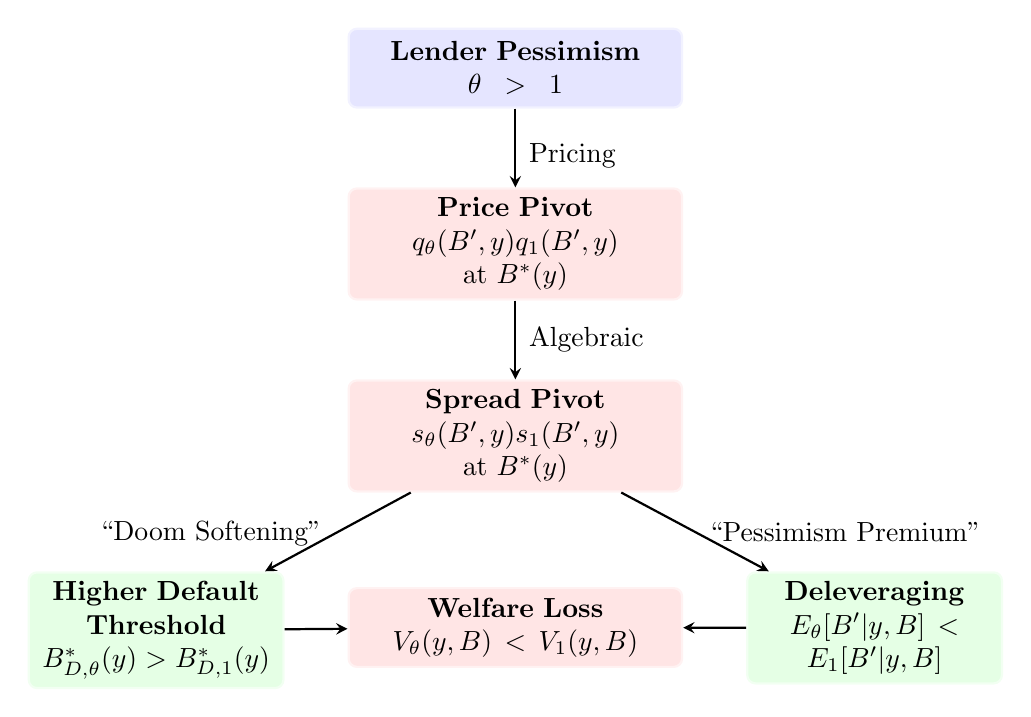
\begin{tikzpicture}[
			node distance=1cm and 1.5cm,
			every node/.style={text centered, minimum height=0.8cm},
			box/.style={rectangle, draw=blue!5, thick, fill=blue!10,text width=4cm, minimum height=1cm, rounded corners=3pt},
			arrow/.style={->, thick, >=stealth},
			effect/.style={rectangle, draw=red!5, thick, fill=red!10, text width=4cm, minimum height=1cm, rounded corners=3pt},
			outcome/.style={rectangle, draw=green!5, thick, fill=green!10, text width=3cm, minimum height=1cm, rounded corners=3pt}
		]

		% Initial shock
		\node[box] (shock) {\textbf{Lender Pessimism} \\ $\theta > 1$};

		% Market effects
		\node[effect, below=of shock] (pivot) {\textbf{Price Pivot} \\ $q_\theta(B',y) \gtrless q_1(B',y)$ \\ at $B^*(y)$};

		\node[effect, below=of pivot] (spread) {\textbf{Spread Pivot} \\ $s_\theta(B',y) \lessgtr s_1(B',y)$ \\ at $B^*(y)$};

		% Policy responses (left and right)
		\node[outcome, below left=1cm and 0.8cm of spread] (threshold) {\textbf{Higher Default} \\ \textbf{Threshold} \\ $B^*_{D,\theta}(y) > B^*_{D,1}(y)$};

		\node[outcome, below right=1cm and 0.8cm of spread] (deleverage) {\textbf{Deleveraging} \\ $\mathbb{E}_\theta[B'|y,B] <$ \\ $\mathbb{E}_1[B'|y,B]$};

		% Final outcome
		\node[effect, below=1.2cm of spread] (welfare) {\textbf{Welfare Loss} \\ $V_\theta(y,B) < V_1(y,B)$};

		% Arrows
		\draw[arrow] (shock) -- (pivot);
		\draw[arrow] (pivot) -- (spread);
		\draw[arrow] (spread) -- (threshold);
		\draw[arrow] (spread) -- (deleverage);
		\draw[arrow] (threshold) -- (welfare);
		\draw[arrow] (deleverage) -- (welfare);

		% Labels on arrows
		\node[right=0.05cm] at ($(shock)!0.5!(pivot)$) {Pricing};
		\node[right=0.05cm] at ($(pivot)!0.5!(spread)$) {Algebraic};
		\node[left=0.05cm] at ($(spread)!0.5!(threshold)$) {``Doom Softening''};
		\node[right=0.05cm] at ($(spread)!0.5!(deleverage)$) {``Pessimism Premium''};

	\end{tikzpicture}
	\caption{The Causal Chain of Lender Pessimism}
	\label{fig:causal_chain}
	\parbox{\linewidth}{\small\textit{Note:} This diagram illustrates how a single behavioral friction ($\theta > 1$) propagates through the economy. Lender pessimism first alters market pricing, creating a pivoting bond price schedule. The sovereign optimally responds to this new environment, but cannot fully escape the welfare costs of dealing with biased lenders.}
\end{figure}
To crystallize the novel contributions of this behavioral channel, Table
\ref{tab:prediction_comparison} explicitly contrasts the key predictions of the
pessimism model with those of a standard reputation model.

\begin{table}[h!]
	\centering
	\caption{Theoretical Predictions: Pessimism vs. Reputation}
	\label{tab:prediction_comparison}
	\begin{tabularx}{\textwidth}{@{}lXX@{}}
		\toprule
		Prediction Dimension                 & Reputation Model \citep{ColeDowEnglish1995, MorelliMoretti2023} & Pessimism Model (This Paper)                  \\ \midrule
		Price Curve, $q$                     & Monotonically \textit{lower}                                    & \textit{Pivots} around baseline ($q_1$)       \\
		Default Threshold, $B^*_D$           & \textit{Lower}                                                  & \textit{Higher}: $B^*_{D,\theta} > B^*_{D,1}$ \\
		Expected Borrowing, $\mathbb{E}[B']$ & \textit{Lower} (Constraint-driven)                              & \textit{Lower} (Price-driven)                 \\
		Average Spread, $\mathbb{E}[s]$      & \textit{Higher}                                                 & \textit{Higher}                               \\ \bottomrule
	\end{tabularx}
	\parbox{\linewidth}{\small\textit{Note:} This table compares the main theoretical predictions of a standard model where lenders learn about the sovereign's hidden type (reputation) with the behavioral model in this paper where lenders are systematically pessimistic about policy randomness. The bolded items highlight the unique and often counter-intuitive predictions of the pessimism model.}
\end{table}

\section{Quantitative Analysis}
\label{sec:quant}

In this section, I describe the quantitative implementation of the model. I
first outline the calibration of the model parameters and the numerical
strategy used to solve for the equilibrium. Then, I present the business cycle
properties generated by the baseline model and show that it successfully
replicates key features of emerging market economies.

\subsection{Calibration and Numerical Solution}

\paragraph{Calibration}
The model is calibrated at a quarterly frequency. The parameter values are
chosen to be consistent with the sovereign default literature and to broadly
match the macroeconomic features of a typical emerging economy, such as
Argentina. The parameters are summarized in Table~\ref{tab:calibration}.

The preference and endowment parameters are standard. The risk aversion
coefficient $\sigma$ is set to 2. The discount factor $\beta$ is set to 0.9775,
implying an annual real interest rate of approximately 9.5\% when combined with
the model's growth, which is a common value for emerging economies. The
logarithmic endowment process is modeled as an AR (1) with a persistence of
$\rho_y=0.95$ and an innovation standard deviation of $\sigma_y=0.005$.

The debt structure parameters are set to achieve a target Macaulay duration of
5 years (20 quarters) for a risk-free bond, which implies a quarterly principal
decay rate of $\delta=0.04$. The coupon rate $\kappa$ is set to equal
$\delta+r$ so that the price of a risk-free bond is normalized to one. The
probability of re-entering credit markets after a default, $\gamma$, is set to
0.125, implying an average exclusion period of 2 years (8 quarters). The output
cost of default, governed by $\lambda_0$ and $\lambda_1$, is specified to be
nonlinear, consistent with the findings of
\citep{ChatterjeeEyigungor2012}.\footnote{The specific values are $\lambda_0 =
		-0.48$ and $\lambda_1 = 0.525$, calibrated to match the severity and shape of
	output losses observed in historical default episodes.}

The scale parameters of the Gumbel taste shocks, $\eta$ and $\rho$, are set to
small values to ensure that decisions are primarily driven by economic
fundamentals, while still ensuring the stability and tractability of the
numerical solution.\footnote{Specifically, $\eta = 5 \times 10^{-4}$ for
	default decisions and $\rho = 1 \times 10^{-5}$ for borrowing decisions. These
	small values maintain the primacy of economic fundamentals while providing
	computational tractability through the log-sum-exp formulation.}

\begin{table}[h!]
	\centering
	\caption{Baseline Calibration (Quarterly)}
	\label{tab:calibration}
	\begin{tabular}{@{}lll@{}}
		\toprule
		Parameter              & Value              & Description                                  \\ \midrule
		\multicolumn{3}{l}{\textit{Preferences and Endowments}}                                    \\
		$\sigma$               & 2.0                & CRRA coefficient of relative risk aversion   \\
		$\beta$                & 0.9775             & Sovereign's discount factor                  \\
		$\rho_y$               & 0.95               & Persistence of log endowment AR(1)           \\
		$\sigma_y$             & 0.005              & Std. dev. of endowment innovations           \\
		\multicolumn{3}{l}{\textit{Debt and Default}}                                              \\
		$r$                    & 0.01               & Quarterly risk-free interest rate (4\% ann.) \\
		$\delta$               & 0.04               & Principal decay rate (for 5-year duration)   \\
		$\kappa$               & 0.05               & Coupon rate ($\delta+r$)                     \\
		$\gamma$               & 0.125              & Re-entry probability (avg. 2-year exclusion) \\
		$\lambda_0, \lambda_1$ & -0.48, 0.525       & Output cost function parameters              \\
		\multicolumn{3}{l}{\textit{Computational Parameters}}                                      \\
		$\eta$                 & $5 \times 10^{-4}$ & Scale of default taste shock                 \\
		$\rho$                 & $1 \times 10^{-5}$ & Scale of borrowing taste shock               \\
		$\theta$               & 1.0                & Baseline lender pessimism coefficient        \\ \bottomrule
	\end{tabular}
	\parbox{\linewidth}{\small\textit{Note:} The table presents the parameter values used in the baseline calibration of the model. Parameters are set to match standard values in the sovereign default literature and key macroeconomic features of emerging economies like Argentina.}

	{\color{red}[TODO: Add parameter-target correspondence table showing which parameter targets which moment/statistic, as suggested by reviewer to improve transparency of calibration strategy]}
\end{table}

\paragraph{Numerical Solution}
I solve the model numerically using value function iteration on a discretized
state space. The state space consists of the sovereign's current endowment $y$
and its outstanding debt level $B$.

The endowment process in \eqref{eq:endowment} is discretized into $N_y = 201$
states using Tauchen's method. The state space for debt, $B$, is represented by
a uniform grid of $N_B = 600$ points, ranging from 0 to 75\% of mean output.

The solution method iterates on the value functions ($V, V^D, V^R$) and the
bond price function ($q$) until they converge to a joint fixed point. A key
feature of the numerical strategy is the use of the log-sum-exp formulation for
choices subject to Gumbel taste shocks. This technique replaces the
non-differentiable `max` operator with a smooth, analytical expression, which
greatly improves the stability and speed of the algorithm by obviating the need
for numerical maximization routines at each grid point. For further numerical
robustness, I employ stabilized log-sum-exp implementations that prevent
floating-point overflow and underflow errors that could arise from the small
taste shock parameters.\footnote{ A detailed discussion of these numerical
	stability techniques is provided in Appendix~\ref{app:numerical_stability}.
}The entire solution algorithm is implemented in Fortran and parallelized using
OpenMP to leverage multi-core processors.

\subsection{Business Cycle Implications of Lender Pessimism}

To understand the quantitative implications of lender pessimism, I simulate the
model under three scenarios: the baseline rational-expectations benchmark
($\theta=1$), a medium-pessimism case ($\theta=10$), and a high-pessimism case
($\theta=100$).\footnote{The choice of $\theta=10$ and $\theta=100$ as medium
	and high pessimism cases is motivated by the need to demonstrate clear
	quantitative differences while maintaining computational tractability.
	Intermediate values such as $\theta=30$ or $\theta=50$ could also be examined
	to show the continuous nature of the relationship.} Table
\ref{tab:main_results} reports the key business cycle moments from these
simulations, revealing how pessimism reshapes macroeconomic behavior.

\paragraph{The Rational Benchmark}
The baseline model with rational lenders ($\theta=1$) successfully generates
results that are broadly consistent with the stylized facts for emerging
economies. The average debt-to-GDP ratio is a moderate 7.90\%, and the
sovereign pays an average annualized credit spread of 2.00\%. Consistent with
the empirical literature, the model produces consumption that is more volatile
than output, counter-cyclical credit spreads (correlation of -0.43 with
ln(GDP)), and a slightly counter-cyclical trade balance. When output falls,
default risk rises, increasing spreads; simultaneously, the government attempts
to borrow to smooth the shock, worsening the trade balance. These features
confirm that the model provides a standard and reasonable benchmark against
which to evaluate the effects of pessimism.

\paragraph{Deleveraging and the Price of Fear}
The introduction of lender pessimism dramatically alters these outcomes, but in
a non-linear fashion. Under moderate pessimism ($\theta=10$), the sovereign's
average debt level (5.53\%) and borrowing cost (2.75\%) remain remarkably close
to the baseline. However, a shift to high pessimism ($\theta=100$) triggers a
stark deleveraging and a significant increase in average borrowing costs. The
mean debt-to-GDP ratio falls precipitously by nearly 5 percentage points to
just 2.70\%. This is a direct consequence of the market discipline predicted in
Proposition~\ref{prop:deleveraging}: faced with worse prices in the primary
borrowing region, the sovereign optimally reduces its debt issuance. However,
this conservative policy does not earn it lower interest rates. Instead, the
average credit spread more than doubles to 4.15\%. This result---deleveraging
in the face of even higher average spreads—starkly illustrates the power of the
behavioral bias. In a pure reputation model, deleveraging should lower risk and
borrowing costs; here, it is a constrained-optimal response to the ``pessimism
premium,'' a penalty the sovereign can never fully escape simply by reducing
its debt. Lenders demand substantial compensation for the perceived risk of an
``out of the blue'' default, an effect that overwhelms the fact that the
sovereign is, in reality, safer due to its lower debt level.

\paragraph{Amplified Financial Cycles}
Pessimism not only raises the level of borrowing costs but also progressively
amplifies their cyclicality. The correlation between credit spreads and GDP
becomes more negative as pessimism increases, moving from -0.43 in the baseline
to -0.80 under moderate pessimism, and then sharply to -0.89 in the
high-pessimism case. This indicates that financial conditions become
exquisitely sensitive to fluctuations in the country's income. When a negative
shock hits, pessimistic lenders' fears are magnified, leading to a much sharper
spike in spreads than would occur in a rational market. This tightening of
financial conditions occurs precisely when the sovereign needs market access
the most, exacerbating the downturn and making financial markets a powerful
source of procyclical shocks rather than a tool for macroeconomic
stabilization.

\paragraph{An Illusion of Stability}
Interestingly, the volatility of both the debt-to-GDP ratio and credit spreads
decreases as pessimism rises. This is not a sign of improved stability but
rather a mechanical result of the sovereign's forced deleveraging, creating an
\textit{illusion of financial stability}. By maintaining a lower average debt
level, the sovereign operates further away from its default threshold (which,
paradoxically, is higher, per Proposition~\ref{prop:threshold}). This reduces
the frequency of episodes of high debt and soaring spreads, leading to lower
overall volatility in these financial variables, even as the average spread
remains high. Despite these large changes in financial markets, the impact on
consumption volatility is minimal. The sovereign adapts to the harsher
borrowing environment by reducing its reliance on foreign debt for consumption
smoothing, effectively trading away the benefits of international financial
integration for a quieter, but more expensive, life.

\begin{table}[h]
	\centering
	\caption{Business Cycle Implications of Lender Pessimism}
	\label{tab:main_results}
	\begin{tabular}{@{}lccc@{}}
		\toprule
		Moment                               & Baseline ($\theta=1$) & Med. ($\theta=10$) & High  ($\theta=100$) \\ \midrule
		\multicolumn{3}{l}{\textit{Mean and Volatility}}                                                         \\
		Mean Debt-to-GDP Ratio (\%)          & 7.90                  & 5.53               & 2.70                 \\
		Std. Dev. of Debt-to-GDP Ratio (\%)  & 0.87                  & 0.85               & 0.74                 \\
		Mean Spread (annualized, \%)         & 2.00                  & 2.75               & 4.15                 \\
		Std. Dev. of Spread (annualized, \%) & 0.77                  & 0.49               & 0.58                 \\
		Std. Dev. of ln(Consumption) (\%)    & 3.48                  & 3.53               & 3.41                 \\
		Std. Dev. of ln(GDP) (\%)            & 3.04                  & 3.19               & 3.19                 \\
		Mean Trade Balance/GDP (\%)          & 0.42                  & 0.32               & 0.18                 \\
		Std. Dev. of Trade Balance/GDP (\%)  & 0.51                  & 0.43               & 0.32                 \\
		\multicolumn{3}{l}{\textit{Correlations}}                                                                \\
		Corr(Spread, ln(GDP))                & -0.43                 & -0.80              & -0.89                \\
		Corr(Trade Balance/GDP, ln(GDP))     & -0.28                 & -0.28              & -0.26                \\
		Corr(Debt/GDP, ln(GDP))              & 0.70                  & 0.79               & 0.84                 \\ \bottomrule
	\end{tabular}
	\parbox{\linewidth}{\small\textit{Note:} The table reports moments from a long simulation of the model (100,000 periods after a 1,000-period burn-in). Spreads are annualized. All other variables are in quarterly terms.}

	{\color{red}[TODO: Add robustness checks showing results remain consistent under longer simulations and different random seeds]}
\end{table}

\subsection{The Mechanics of Pessimism: Distributions and Policy Functions}

\paragraph{Long-Run Outcomes: A Shift in Distributions}
The aggregate business cycle statistics in Table~\ref{tab:main_results} are the
result of fundamental shifts in the sovereign's equilibrium behavior, which are
best understood by examining the model's policy functions and resulting
stationary distributions. Figure~\ref{fig:sim_distributions} plots the
simulated histograms for debt and credit spreads, revealing the long-run
consequences of lender pessimism. Panel (a) starkly illustrates the
deleveraging predicted by Proposition~\ref{prop:deleveraging}. The entire
distribution of the debt-to-GDP ratio shifts dramatically to the left,
representing a strategic retreat from international capital markets. This is
not an arbitrary choice but the sovereign's optimal response to the punitive
pricing it faces. Faced with a market that consistently overestimates its risk,
the government is disciplined into a permanently more conservative fiscal
stance.

This retreat, however, does not earn the sovereign better credit terms. Panel
(b) reveals the central paradox: as the sovereign deleverages, its average
borrowing cost increases. The entire distribution of credit spreads is pushed
to the right. This is the tangible result of the "pessimism premium" described
in Corollary~\ref{cor:spread_pivot}. The sovereign is forced into a low-debt
trap where, despite being fundamentally safer due to its lower leverage, it
faces a persistently higher cost of capital because lenders' pessimistic
beliefs dominate their assessment of fundamentals.

\begin{figure}[h!]
	\centering
	\begin{subfigure}[b]{0.48\textwidth}
		\centering
		\includegraphics[width=\textwidth]{../../pessimism-default-model/results/comparison_figure_7.pdf}
		\caption{Debt-to-GDP Ratio Distribution}
		\label{fig:dist_debt}
	\end{subfigure}
	\hfill
	\begin{subfigure}[b]{0.48\textwidth}
		\centering
		\includegraphics[width=\textwidth]{../../pessimism-default-model/results/comparison_figure_6.pdf}
		\caption{Credit Spread Distribution}
		\label{fig:dist_spread}
	\end{subfigure}
	\caption{Simulated Stationary Distributions}
	\label{fig:sim_distributions}
	\parbox{\linewidth}{\small\textit{Note:} The distributions are generated from a long simulation of the model (100,000 periods). The figure shows how rising lender pessimism progressively shifts the long-run distribution of the debt-to-GDP ratio to the left (deleveraging) and the credit spread distribution to the right (higher borrowing costs).}
\end{figure}

\paragraph{State-Contingent Policies: The Pivoting Effect}
The long-run distributional shifts are driven by state-by-state changes in the
sovereign's optimal policies, which are themselves a reaction to the altered
price schedule. Figure~\ref{fig:policy_pivot} visualizes how pessimism causes
key functions to "pivot" around the rational benchmark, providing a graphical
confirmation of the paper's central theoretical results.

Panels~\ref{fig:pivot_price} and~\ref{fig:pivot_spread} illustrate the core
price pivot. At low debt levels, where a rational lender sees little risk, the
pessimistic lender prices in the possibility of an "out of the blue" default,
leading to lower prices and higher spreads. At very high debt levels, where a
rational lender sees default as nearly certain, the pessimistic lender's belief
in randomness allows for a small chance of an "irrational" repayment, leading
to paradoxically better terms (the "softening of doom" effect). This pivot in
the price schedule is the key external force acting on the sovereign, and it
offers a richer dynamic than the simple downward price shift one would expect
from a pure reputation loss.

Panels~\ref{fig:pivot_default} and~\ref{fig:pivot_borrowing} show the
sovereign's endogenous response. The government internalizes the new price
schedule. The better terms available in the high-debt region increase the value

of maintaining market access, making the sovereign more resilient and pushing
out its default threshold (Proposition~\ref{prop:threshold}). More importantly,
in the normal course of borrowing, the sovereign faces worse prices, which act
as a higher effective cost of capital. The optimal response, shown in Panel
\ref{fig:pivot_borrowing}, is to deleverage and choose a lower next-period debt
level for any given state (Proposition~\ref{prop:deleveraging}).

\begin{figure}[h!]
	\centering
	\begin{subfigure}[b]{0.48\textwidth}
		\centering
		\includegraphics[width=\textwidth]{../../pessimism-default-model/results/comparison_figure_3.pdf}
		\caption{Bond Price Schedule, $q(B',y)$}
		\label{fig:pivot_price}
	\end{subfigure}
	\hfill
	\begin{subfigure}[b]{0.48\textwidth}
		\centering
		\includegraphics[width=\textwidth]{../../pessimism-default-model/results/comparison_figure_4.pdf}
		\caption{Credit Spread, $s(B',y)$}
		\label{fig:pivot_spread}
	\end{subfigure}
	\vskip\baselineskip
	\begin{subfigure}[b]{0.48\textwidth}
		\centering
		\includegraphics[width=\textwidth]{../../pessimism-default-model/results/comparison_figure_2.pdf}
		\caption{Default Probability, $P(d=1|B,y)$}
		\label{fig:pivot_default}
	\end{subfigure}
	\hfill
	\begin{subfigure}[b]{0.48\textwidth}
		\centering
		\includegraphics[width=\textwidth]{../../pessimism-default-model/results/comparison_figure_9.pdf}
		\caption{Borrowing Policy, $\mathbb{E}[B'|B,y]$}
		\label{fig:pivot_borrowing}
	\end{subfigure}
	\caption{Policy Function Pivoting}
	\label{fig:policy_pivot}
	\parbox{\linewidth}{\small\textit{Note:} The plots show the key policy and pricing functions for three different levels of endowment y (low, medium, and high). The functions for the baseline ($\theta=1$, dashed), medium pessimism ($\theta=10$, dash-dot), and high pessimism ($\theta=100$, solid) cases are shown. Rising pessimism causes the functions to pivot.}
\end{figure}

\paragraph{Welfare Consequences}
The sovereign's policy adjustments—deleveraging and tolerating higher debt
before default—are optimal given the market it faces, but they cannot overcome
the fundamental handicap of dealing with paranoid lenders. Proposition
\ref{prop:welfare} predicted a direct welfare loss, a result powerfully
confirmed by Figure~\ref{fig:welfare_loss}. The sovereign's value function is
uniformly and significantly lower in the pessimistic economy.

This welfare loss stems from the impairment of the sovereign's ability to
smooth consumption. Access to international credit markets is a tool to buffer
domestic shocks. Pessimism effectively places a tax on the use of this tool. By
making borrowing more expensive in the relevant range, it forces the sovereign
to either endure more volatile consumption or to self-insure by maintaining an
inefficiently low level of debt. The ``benefit'' of better prices in the
far-off, high-risk region is an option that is too remote and uncertain to
compensate for the persistent, day-to-day welfare losses incurred from being
forced to transact with a market that systematically overestimates its
propensity to fail.

\begin{figure}[h!]
	\centering
	\includegraphics[width=0.6\textwidth]{../../pessimism-default-model/results/comparison_figure_1.pdf}
	\caption{Welfare Loss}
	\label{fig:welfare_loss}
	\parbox{\linewidth}{\small\textit{Note:} The figure plots the sovereign's ex-ante value function $V(y, B)$ for the baseline ($\theta=1$, dashed), medium pessimism ($\theta=10$, dash-dot), and high pessimism ($\theta=100$, solid) economies. The value function is uniformly lower under higher degrees of pessimism, indicating a progressive welfare loss.}
\end{figure}

\subsection{Dynamic Responses and Adjustment Paths}

The dynamic implications of lender pessimism reveal how pessimism affects the
sovereign's adjustment paths and responses to shocks.

\paragraph{Deleveraging Dynamics: The Transition to Lower Debt}

Figure~\ref{fig:deleveraging_paths} traces optimal debt adjustment paths under
different initial conditions and degrees of lender pessimism. Consistent with
Proposition~\ref{prop:deleveraging}, economies with higher pessimism
systematically converge to lower debt levels regardless of starting point.
Remarkably, even from low initial debt, the high-pessimism economy continues
deleveraging, representing a fundamental fiscal shift rather than temporary
adjustment.

The consumption and spread dynamics reveal important adjustment costs.
Panel~\ref{fig:consumption_path} shows that high-pessimism economies experience
more volatile consumption during deleveraging despite ultimately achieving
lower debt. Panel~\ref{fig:spread_path_delev} demonstrates that spreads remain
persistently elevated throughout adjustment, confirming that the ``pessimism
premium'' reflects systematic risk overestimation at all debt levels rather
than just current leverage.

\begin{figure}[h]
	\centering
	\begin{subfigure}[b]{0.48\textwidth}
		\centering
		\includegraphics[width=\textwidth]{../../pessimism-default-model/results/comparison_figure_11.pdf}
		\caption{Debt}
		\label{fig:debt_path}
	\end{subfigure}
	\hfill
	\begin{subfigure}[b]{0.48\textwidth}
		\centering
		\includegraphics[width=\textwidth]{../../pessimism-default-model/results/comparison_figure_12.pdf}
		\caption{Consumption}
		\label{fig:consumption_path}
	\end{subfigure}
	\vskip\baselineskip
	\begin{subfigure}[b]{0.48\textwidth}
		\centering
		\includegraphics[width=\textwidth]{../../pessimism-default-model/results/comparison_figure_21.pdf}
		\caption{Spread}
		\label{fig:spread_path_delev}
	\end{subfigure}
	\caption{Deleveraging Dynamics}
	\label{fig:deleveraging_paths}
	\parbox{\linewidth}{\small\textit{Note:} The figure shows optimal adjustment paths over 6 quarters starting from three different initial debt levels (low, medium, high) for each degree of lender pessimism. The paths demonstrate how pessimism leads to systematic deleveraging that persists regardless of initial conditions, accompanied by persistently higher spreads and more volatile consumption during the transition.}
\end{figure}

\paragraph{Impulse Response Functions: Shock Propagation under Pessimism}

I examine responses to transitory and persistent productivity shocks (AR(1)
with $\rho = 0.8$) to understand how lender pessimism affects the sovereign's
shock absorption capacity.

\subparagraph{Transitory Shock Responses.} Figure~\ref{fig:irf_transitory} shows responses to a 3\% positive productivity
shock lasting one quarter. While output effects are identical by construction
(panel~\ref{fig:irf_trans_output}), pessimism fundamentally alters other
responses. High-pessimism economies exhibit muted debt reduction
(panel~\ref{fig:irf_trans_debt}) and consumption smoothing responses
(panel~\ref{fig:irf_trans_consumption}), illustrating impaired ability to
exploit temporary favorable conditions. Despite facing identical shocks, these
economies cannot fully capitalize on good fortune due to persistently
unfavorable credit pricing. Spreads fall in all economies
(panel~\ref{fig:irf_trans_spread}), but high-pessimism economies maintain
higher levels throughout adjustment.

\begin{figure}[h]
	\centering
	\begin{subfigure}[b]{0.48\textwidth}
		\centering
		\includegraphics[width=\textwidth]{../../pessimism-default-model/results/comparison_figure_13.pdf}
		\caption{Output}
		\label{fig:irf_trans_output}
	\end{subfigure}
	\hfill
	\begin{subfigure}[b]{0.48\textwidth}
		\centering
		\includegraphics[width=\textwidth]{../../pessimism-default-model/results/comparison_figure_14.pdf}
		\caption{Debt}
		\label{fig:irf_trans_debt}
	\end{subfigure}
	\vskip\baselineskip
	\begin{subfigure}[b]{0.48\textwidth}
		\centering
		\includegraphics[width=\textwidth]{../../pessimism-default-model/results/comparison_figure_15.pdf}
		\caption{Consumption}
		\label{fig:irf_trans_consumption}
	\end{subfigure}
	\hfill
	\begin{subfigure}[b]{0.48\textwidth}
		\centering
		\includegraphics[width=\textwidth]{../../pessimism-default-model/results/comparison_figure_16.pdf}
		\caption{Spread}
		\label{fig:irf_trans_spread}
	\end{subfigure}
	\caption{Impulse Responses to Transitory Productivity Shock}
	\label{fig:irf_transitory}
	\parbox{\linewidth}{\small\textit{Note:} The figure shows responses to a 3\% positive productivity shock that lasts for one quarter. All variables are expressed as percentage deviations from their respective steady states (spreads in basis points). The responses demonstrate how lender pessimism constrains the sovereign's ability to take advantage of temporary favorable conditions.}
\end{figure}

\subparagraph{Persistent Shock Responses.} Figure~\ref{fig:irf_persistent} shows responses to persistent productivity
shocks ($\rho = 0.8$). Persistence matters more for high-pessimism economies,
which exhibit more pronounced and sustained debt reduction
(panel~\ref{fig:irf_pers_debt}) as sovereigns recognize rare opportunities to
escape the ``high-spread trap.'' While persistent shocks enable better
consumption smoothing across all economies
(panel~\ref{fig:irf_pers_consumption}), high-pessimism economies still
underperform due to fundamental impairment of consumption insurance. Spread
responses (panel~\ref{fig:irf_pers_spread}) are more persistent than in the
transitory case, but high-pessimism economies maintain higher levels throughout
adjustment.

\begin{figure}[h]
	\centering
	\begin{subfigure}[b]{0.48\textwidth}
		\centering
		\includegraphics[width=\textwidth]{../../pessimism-default-model/results/comparison_figure_17.pdf}
		\caption{Output}
		\label{fig:irf_pers_output}
	\end{subfigure}
	\hfill
	\begin{subfigure}[b]{0.48\textwidth}
		\centering
		\includegraphics[width=\textwidth]{../../pessimism-default-model/results/comparison_figure_18.pdf}
		\caption{Debt}
		\label{fig:irf_pers_debt}
	\end{subfigure}
	\vskip\baselineskip
	\begin{subfigure}[b]{0.48\textwidth}
		\centering
		\includegraphics[width=\textwidth]{../../pessimism-default-model/results/comparison_figure_19.pdf}
		\caption{Consumption}
		\label{fig:irf_pers_consumption}
	\end{subfigure}
	\hfill
	\begin{subfigure}[b]{0.48\textwidth}
		\centering
		\includegraphics[width=\textwidth]{../../pessimism-default-model/results/comparison_figure_20.pdf}
		\caption{Spread}
		\label{fig:irf_pers_spread}
	\end{subfigure}
	\caption{Impulse Responses to Persistent Productivity Shock}
	\label{fig:irf_persistent}
	\parbox{\linewidth}{\small\textit{Note:} The figure shows responses to a 3\% productivity shock with autocorrelation $\rho = 0.8$. All variables are expressed as percentage deviations from steady state (spreads in basis points). The persistent nature of the shock reveals how lender pessimism constrains fiscal flexibility even during extended periods of favorable fundamentals.}
\end{figure}

\paragraph{Implications}

The dynamic analysis reveals three fundamental economic mechanisms. First,
deleveraging under pessimism creates persistent allocative distortions—the
adjustment process itself becomes a source of inefficiency as elevated spreads
persist throughout transition, generating deadweight losses that compound over
time. This represents a departure from standard models where adjustment costs
are temporary. Second, pessimism creates asymmetric shock transmission:
sovereigns experience constrained benefits from favorable shocks while facing
amplified costs from adverse ones, fundamentally altering the risk-return
profile of sovereign borrowing. This asymmetry suggests that traditional
moments-based calibrations may understate welfare costs. Finally, the
interaction between persistence and beliefs generates hysteresis effects:
temporary improvements in fundamentals produce limited deleveraging, while
sustained improvements are necessary to overcome entrenched pessimistic priors.

\section{Extensions}

\subsection{Theoretical Extensions}

\paragraph{Ramsey Planning Under Pessimism}\label{sec:ramsey}

While Proposition~\ref{prop:welfare} establishes that lender pessimism
generates a welfare loss, a natural question arises: could this loss be
mitigated through optimal fiscal policy? To address this, I consider a Ramsey
planner \citep{LucasStokey1983} who can use lump-sum taxes and transfers but
cannot alter the bond pricing mechanism. This extension formalizes the
intuition that pessimism creates a fundamental allocative distortion beyond
simple income effects \citep{ChariKehoe1999}.

\textit{Economic Intuition}: The key insight is that lender pessimism operates as a persistent ``tax'' on borrowing that distorts intertemporal prices. While a Ramsey planner can use lump-sum transfers to redistribute resources optimally within any given period, they cannot fix the distorted shadow prices that guide borrowing decisions. The pessimistic price schedule makes debt artificially expensive in safe states, leading to suboptimal savings and borrowing patterns. This creates a dynamic inefficiency that fiscal transfers cannot address---the government faces the wrong intertemporal trade-offs when deciding how much to borrow across different states of nature.

Let the Ramsey planner's problem be to choose consumption allocations $\{c_t\}$
and debt policies $\{B_{t+1}\}$ to maximize the sovereign's welfare, subject to
the resource constraint modified by lump-sum transfers $\tau_t$\footnote{While
	the baseline model is formulated as a Recursive Markov Perfect Equilibrium with
	stationary value functions $V(y,B)$, the extensions in this section use
	time-indexed notation $\{c_t, B_t, \theta_t\}$ to analyze dynamic processes.
	This notation is equivalent to the recursive formulation: each period's
	equilibrium state $(y_t, B_t)$ corresponds to the recursive state variables,
	and the time-indexed sequences represent equilibrium paths under the recursive
	decision rules. The time subscripts facilitate the analysis of belief updating,
	learning dynamics, and intertemporal policy choices while maintaining
	consistency with the underlying Markov structure.}:
\begin{equation}
	c_t + \kappa B_t + \tau_t = y_t + [B_{t+1} - (1-\delta)B_t]q_\theta(y_t, B_{t+1}) \label{eq:ramsey_constraint}
\end{equation}
where the planner is constrained to use the pessimistic price schedule $q_\theta(\cdot)$ but can choose transfers to achieve first-best consumption smoothing.

\begin{proposition}\label{prop:ramsey_welfare}
	Define $W^R_i$ as the value of the Ramsey planner's problem under price schedule $q_i(\cdot)$:
	\begin{equation}
		W^R_i = \max_{\{c_t, B_{t+1}, \tau_t\}_{t=0}^\infty} \mathbb{E}_0 \left[ \sum_{t=0}^\infty \beta^t u(c_t) \right] \label{eq:ramsey_welfare_def}
	\end{equation}
	subject to \eqref{eq:ramsey_constraint} and $\mathbb{E}_0 \left[ \sum_{t=0}^\infty \frac{\tau_t}{\prod_{s=1}^t (1+r_s)} \right] = 0$.

	Even under optimal Ramsey planning with lump-sum transfers, the welfare loss
	from lender pessimism persists:
	\begin{equation}
		W^R_\theta < W^R_1 \label{eq:ramsey_welfare_loss}
	\end{equation}
\end{proposition}

\begin{proof}
	See Appendix \ref{app:proof_ramsey}.
\end{proof}
The intuition is that while the Ramsey planner can use transfers to achieve
optimal consumption levels \textit{conditional on debt choices}, the
pessimism-distorted price schedule still leads to suboptimal debt decisions.
The planner faces the wrong intertemporal prices and thus makes allocatively
inefficient borrowing choices, creating deadweight loss that transfers cannot
eliminate \citep{AiyagariMarcetSargentSeppala2002}. Economically, this demonstrates that even omnipotent fiscal policy cannot undo the damage from mispricing in international capital markets---pessimism creates a wedge between social and private returns to borrowing that persists regardless of domestic redistribution. While this analysis takes the pessimistic beliefs as given, a natural extension is to endogenize their formation through learning processes, building on the literature of model uncertainty and robustness \citep{HansenSargent2001}.

\paragraph{Endogenous Belief Formation}

Consider an extension where lenders form beliefs about the taste shock
volatility parameter $\theta$ through Bayesian learning
\citep{CogleySargent2008}. Let $\theta_t$ denote the lenders' perceived
volatility parameter in period $t$, where $\theta_t \in [\underline{\theta},
		\bar{\theta}]$ with $\underline{\theta} = 1$ (correct beliefs) and
$\bar{\theta} > 1$ (maximum pessimism).

\textit{Economic Intuition}: This extension addresses a natural question: if lenders are rational learners, shouldn't pessimistic beliefs eventually be corrected by experience? The answer hinges on psychological biases in information processing. Even rational Bayesian learners can maintain persistent pessimism if they exhibit ``negativity bias''---overweighting negative surprises relative to positive ones. When defaults occur unexpectedly (relative to their models), lenders update their beliefs more dramatically than when repayments exceed expectations. This asymmetric learning mechanism, well-documented in behavioral psychology, can cause pessimistic beliefs to become self-reinforcing: bad news matters more than good news, creating a ratchet effect where beliefs drift toward pessimism over time.

Lenders observe the sovereign's default decisions $\{d_s\}_{s=0}^{t-1}$ and
update their beliefs according to:
\begin{equation}
	\theta_{t+1} = \lambda \theta_t + (1-\lambda) \hat{\theta}(\{d_s\}_{s=0}^t) \label{eq:belief_updating}
\end{equation}
where $\lambda \in (0,1)$ captures persistence in beliefs and $\hat{\theta}(\cdot)$ is the maximum likelihood estimator of $\theta$ given observed default patterns.

Define the \textit{surprise intensity} of a default in state $(y,B)$ as:
\begin{equation}
	\xi(y,B) = \max\left\{0, \frac{P_1(y,B) - P_{\theta_t}(y,B)}{P_1(y,B)}\right\} \label{eq:surprise_intensity}
\end{equation}
where $P_\theta(y,B)$ is the default probability under parameter $\theta$. The belief updating mechanism exhibits \textit{negativity bias} \citep{BaumeisterBratslavskyFinkenauer2001}: lenders overweight surprising defaults relative to surprising repayments, consistent with the literature on overreaction to salient events \citep{BordaloGennaioli​Shleifer2018}.

\begin{proposition}\label{prop:endogenous_beliefs}
	Under negativity bias in belief updating, there exists a stationary distribution $\Theta^*$ of beliefs with the following properties:
	\begin{enumerate}
		\item[\textbf{(i)}] \textbf{Persistent Pessimism}: $\mathbb{E}[\theta] > 1$ for all $\theta_0 \in [\underline{\theta}, \bar{\theta}]$.
		\item[\textbf{(ii)}] \textbf{History Dependence}: The long-run belief distribution depends on the realized default history, with $\Theta^*$ first-order stochastically dominating the rational benchmark.
		\item[\textbf{(iii)}] \textbf{Slow Convergence}: The convergence rate to $\Theta^*$ satisfies $\|\theta_t - \mathbb{E}[\Theta^*]\| = O(\lambda^t)$ with $\lambda$ close to 1 when defaults are rare.
	\end{enumerate}
\end{proposition}

\begin{proof}
	See Appendix~\ref{app:proof_endogenous_beliefs}.
\end{proof}

The economic implications are striking: even with rational learning, lenders
can remain systematically pessimistic in the long run. The negativity bias acts
like a ``pessimism trap'' where bad news sticks while good news fades, causing
beliefs to drift away from rationality. This provides a microfoundation for why
sovereign risk premia can remain elevated for extended periods even when
fundamentals improve. The slow convergence result (part iii) captures the idea
that once pessimistic beliefs become entrenched, they are slow to reverse,
consistent with the observed persistence of sovereign risk episodes.

Given that pessimistic beliefs can become entrenched through this learning
mechanism, governments may seek to mitigate their effects through strategic
information disclosure, drawing on insights from the literature on policy
communication \citep{BlinderEhrmannFratzscher2008}.

\paragraph{Optimal Policy Communication}

Consider an extension where the government can choose its transparency level
$\alpha \in [0,1]$, where $\alpha$ represents the precision of public
information about future policy intentions \citep{MorrisShin2002}. Higher
$\alpha$ reduces lenders' perceived uncertainty about taste shocks but may
reveal unfavorable private information, reflecting the optimal information
design trade-offs \citep{AngelosetsPavan2007}.

\textit{Economic Intuition}: This extension recognizes that governments facing pessimistic lenders have an incentive to strategically manage information flows. The key trade-off is between transparency benefits and disclosure costs. By being more transparent about their policy processes, governments can reduce lenders' uncertainty about the true volatility of policy decisions, potentially countering pessimistic beliefs. However, transparency is costly---it requires institutional investments, may reveal unfavorable private information, and constrains future policy flexibility. The optimal transparency choice balances these costs against the benefit of reduced borrowing costs from less pessimistic lenders.

The sovereign's period utility becomes:
\begin{equation}
	u(c,\alpha) = \frac{c^{1-\sigma}}{1-\sigma} - \phi(\alpha) \label{eq:utility_communication}
\end{equation}
where $\phi(\alpha) = \frac{\gamma \alpha^2}{2}$ represents the cost of transparency (monitoring, reporting, political costs).

Under transparency level $\alpha$, lenders perceive the effective taste shock
volatility as:
\begin{equation}
	\theta_{\text{eff}}(\alpha, \theta) = \alpha \cdot 1 + (1-\alpha) \cdot \theta \label{eq:effective_theta}
\end{equation}
where $\theta > 1$ is the baseline pessimism parameter. Higher transparency reduces the effective bias but is costly.

\begin{proposition}\label{prop:optimal_communication}
	The optimal transparency level $\alpha^*$ satisfies:
	\begin{enumerate}
		\item[\textbf{(i)}] \textbf{Interior Solution}: For $\gamma$ in an intermediate range, $\alpha^* \in (0,1)$ with
		      \begin{equation}
			      \frac{\partial}{\partial \alpha} \mathbb{E}[W(\alpha)] = \gamma \alpha^* \label{eq:foc_transparency}
		      \end{equation}
		      where $W(\alpha)$ is the sovereign's welfare under transparency $\alpha$.
		\item[\textbf{(ii)}] \textbf{Pessimism Amplifies Transparency}: $\frac{\partial \alpha^*}{\partial \theta} > 0$. Higher lender pessimism increases optimal transparency.
		\item[\textbf{(iii)}] \textbf{Welfare Dominance}: Under optimal communication, $W(\alpha^*) > W(0)$ when $\theta > \theta_c$ for some critical threshold $\theta_c > 1$.
	\end{enumerate}
\end{proposition}

\begin{proof}
	See Appendix~\ref{app:proof_optimal_communication}.
\end{proof}

The results reveal several important economic insights. First, the interior
solution (part i) demonstrates that transparency is generally valuable but not
unlimited---governments optimally choose partial rather than complete
transparency. Second, the result that pessimism amplifies transparency (part
ii) shows that transparency becomes more valuable precisely when lenders are
more biased. This creates a natural feedback mechanism: countries with worse
reputations or higher perceived policy uncertainty have stronger incentives to
invest in transparent institutions. Finally, the welfare dominance result (part
iii) confirms that strategic communication can be an effective policy tool, but
only when pessimism is sufficiently severe to justify the costs of
transparency.

\section{Conclusion}

Standard models struggle to explain why emerging economies face persistently
high borrowing costs. This paper develops a quantitative sovereign default
model with a behavioral friction---lender pessimism---to address this puzzle. I
assume lenders systematically overestimate the randomness of the sovereign's
policy choices. Theoretically, this pessimism wedge does not uniformly depress
bond prices but instead \textit{pivots} the price schedule, making debt cheaper
at the edge of default but more expensive in normal times. A rational sovereign
responds to these altered incentives in counterintuitive ways: it tolerates a
higher debt burden before defaulting, yet simultaneously deleverages its
day-to-day borrowing. Quantitatively, the model shows that high pessimism can
force the debt-to-GDP ratio down from 7.90\% to 2.70\%, while more than
doubling the average credit spread from 2.00\% to 4.15\%. This deleveraging
creates an ``illusion of financial stability,'' where observable market
volatility falls even as financial cycles are amplified and the sovereign's
welfare declines.

The theoretical extensions provide additional insights. Even optimal Ramsey
fiscal policy cannot eliminate the welfare costs of pessimism because the
distorted bond pricing creates fundamental allocative distortions that
transfers cannot correct. When beliefs are formed endogenously through Bayesian
learning with negativity bias, pessimistic perceptions become self-reinforcing
and persist over time, explaining why some economies face chronically high
borrowing costs. However, governments can partially mitigate these effects
through strategic policy communication, choosing optimal transparency levels to
reduce perceived uncertainty while managing the costs of information
disclosure. My work thus offers a new, behaviorally-grounded perspective on
sovereign risk, demonstrating how market beliefs can be a fundamental driver of
debt crises and highlighting the importance of optimal policy design in
managing these behavioral frictions.

\clearpage
\appendix

% Reset equation counter and redefine equation numbering for appendices
\setcounter{equation}{0}
\renewcommand{\theequation}{\thesection.\arabic{equation}}

\begin{center}
	\Large \textbf{Appendices for ``Default with Pessimism''}\\
	\vspace{0.5cm}
	\large \textbf{Chen Gao}
	\\
	\large \today
\end{center}

This appendix contains the details of the Gumbel distribution and the proofs
for the lemmas and propositions in the paper. Section~\ref{app:gumbel} contains
the details of the Gumbel distribution. Section~\ref{app:proofs} contains the
proofs for the lemmas and propositions in the paper.
Section~\ref{app:computations} contains the computational algorithm details for
the model, including the numerical stability techniques employed in the
discrete choice implementation.

\section{Gumbel Distribution in Default Models}\label{app:gumbel}
In this section, I provide some useful results about the Gumbel distribution to
help formulate the close form solution presented in Section \ref{sec:model}.

\begin{lemma}
	\label{lem:gumbel_max_expectation}
	Let $\varepsilon_1, \varepsilon_2$ be independent random variables distributed as Gumbel$(-\eta\gamma, \eta)$, where $\gamma$ is the Euler-Mascheroni constant. Let $V_1, V_2 \in \mathbb{R}$ be deterministic constants. Then:
	\begin{equation}
		\mathbb{E}\left[\max\{V_1 + \varepsilon_1, V_2 + \varepsilon_2\}\right] = \eta \ln\left( \exp\frac{V_1}{\eta} + \exp\frac{V_2}{\eta} \right).
	\end{equation}
\end{lemma}

\begin{proof}
	See Appendix~\ref{app:proof_gumbel_max_expectation}.
\end{proof}

\begin{lemma}
	\label{lem:gumbel_logit}
	Let $\varepsilon_1, \varepsilon_2$ be independent Gumbel$(-\eta\gamma, \eta)$ random variables, and let $V_1, V_2 \in \mathbb{R}$ be deterministic values. Then:
	\begin{equation}
		\Pr\{V_1 + \varepsilon_1 > V_2 + \varepsilon_2\} = \frac{\exp\frac{V_1}{\eta}}{\exp\frac{V_1}{\eta} + \exp\frac{V_2}{\eta}}.
	\end{equation}
\end{lemma}

\begin{proof}
	See Appendix~\ref{app:proof_gumbel_logit}.
\end{proof}

\begin{lemma}
	\label{lem:gumbel_multinomial}
	Let $\{V_i\}_{i=1}^n$ be deterministic values and $\{\varepsilon_i\}_{i=1}^n$ be independent Gumbel$(-\sigma\gamma, \sigma)$ random variables. Then:
	\begin{align}
		\mathbb{E}\left[\max_{i \in \{1,\ldots,n\}} \{V_i + \varepsilon_i\}\right]    & = \sigma \ln\left( \sum_{i=1}^n \exp\frac{V_i}{\sigma} \right),       \\
		\Pr\left\{\arg\max_{i \in \{1,\ldots,n\}} \{V_i + \varepsilon_i\} = j\right\} & = \frac{\exp\frac{V_j}{\sigma}}{\sum_{i=1}^n \exp\frac{V_i}{\sigma}}.
	\end{align}
\end{lemma}

\begin{proof}
	See Appendix~\ref{app:proof_gumbel_multinomial}.
\end{proof}

\section{Proofs}\label{app:proofs}
This section contains the proofs for the lemmas and propositions in the paper.

\subsection{Proof of Lemma~\ref{lem:gumbel_max_expectation}}\label{app:proof_gumbel_max_expectation}

\begin{proof}
	Let $X_1 = V_1 + \varepsilon_1$ and $X_2 = V_2 + \varepsilon_2$, where $\varepsilon_1, \varepsilon_2$ are independent Gumbel$(-\eta\gamma, \eta)$ random variables. I derive the expected value $\mathbb{E}[\max\{X_1, X_2\}]$. The CDF of a Gumbel$(\mu, \sigma)$ random variable is $F(x; \mu, \sigma) =
		\exp(-\exp(-(x - \mu)/\sigma))$. For the parametrization Gumbel$(-\eta\gamma,
		\eta)$:
	\begin{equation*}
		F_\varepsilon(x) = \exp\left(-\exp\left(-\frac{x}{\eta} - \gamma\right)\right).
	\end{equation*}
	The CDF of $X_i = V_i + \varepsilon_i$ is obtained by translation:
	\begin{equation*}
		F_{X_i}(x) = F_\varepsilon(x - V_i) = \exp\left(-\exp\left(-\frac{x - V_i}{\eta} - \gamma\right)\right).
	\end{equation*}
	The CDF of $\max\{X_1, X_2\}$ is:
	\begin{align*}
		F_{\max}(x) & = \Pr\{\max\{X_1, X_2\} \leq x\} = \Pr\{X_1 \leq x, X_2 \leq x\}                                                                            \\
		            & = F_{X_1}(x) \cdot F_{X_2}(x)                                                                                                               \\
		            & = \exp\left(-\exp\left(-\frac{x - V_1}{\eta} - \gamma\right)\right) \cdot \exp\left(-\exp\left(-\frac{x - V_2}{\eta} - \gamma\right)\right) \\
		            & = \exp\left(-\exp\left(-\frac{x - V_1}{\eta} - \gamma\right) - \exp\left(-\frac{x - V_2}{\eta} - \gamma\right)\right)                       \\
		            & = \exp\left(-e^{-\gamma}\left(\exp\left(-\frac{x - V_1}{\eta}\right) + \exp\left(-\frac{x - V_2}{\eta}\right)\right)\right).
	\end{align*}
	Let $\tilde{\mu} = \eta \ln\left(\exp\frac{V_1}{\eta} +
		\exp\frac{V_2}{\eta}\right)$. We can rewrite:
	\begin{align*}
		 & \exp\left(-\frac{x - V_1}{\eta}\right) + \exp\left(-\frac{x - V_2}{\eta}\right)                                   \\
		 & = \exp\left(-\frac{x}{\eta}\right)\left(\exp\frac{V_1}{\eta} + \exp\frac{V_2}{\eta}\right)                        \\
		 & = \exp\left(-\frac{x}{\eta}\right) \exp\frac{\tilde{\mu}}{\eta} = \exp\left(-\frac{x - \tilde{\mu}}{\eta}\right).
	\end{align*}
	Therefore,
	\begin{equation*}
		F_{\max}(x) = \exp\left(-e^{-\gamma}\exp\left(-\frac{x - \tilde{\mu}}{\eta}\right)\right) = \exp\left(-\exp\left(-\frac{x - \tilde{\mu}}{\eta} - \gamma\right)\right).
	\end{equation*}
	Thus $\max\{X_1, X_2\}$ follows a Gumbel$(\tilde{\mu} - \eta\gamma, \eta)$
	distribution. Since the expectation of a Gumbel$(\mu, \sigma)$ random variable
	is $\mu + \sigma\gamma$:
	\begin{align*}
		\mathbb{E}[\max\{X_1, X_2\}] & = (\tilde{\mu} - \eta\gamma) + \eta\gamma = \tilde{\mu}             \\
		                             & = \eta \ln\left(\exp\frac{V_1}{\eta} + \exp\frac{V_2}{\eta}\right).
	\end{align*}
\end{proof}

\subsection{Proof of Lemma~\ref{lem:gumbel_logit}}\label{app:proof_gumbel_logit}

\begin{proof}
	Let $X_1 = V_1 + \varepsilon_1$ and $X_2 = V_2 + \varepsilon_2$ as before. I compute $\Pr\{X_1 > X_2\} = \Pr\{\varepsilon_1 - \varepsilon_2 > V_2 - V_1\}$. I first establish that for independent Gumbel$(\mu, \sigma)$ random variables
	$\varepsilon_1$ and $\varepsilon_2$, the difference $\varepsilon_1 -
		\varepsilon_2$ follows a logistic distribution. The CDF of $\varepsilon_i$ is
	$F(x) = \exp(-\exp(-(x-\mu)/\sigma))$. For $Z = \varepsilon_1 - \varepsilon_2$,
	I compute:
	\begin{align*}
		F_Z(z) & = \Pr\{\varepsilon_1 - \varepsilon_2 \leq z\} = \Pr\{\varepsilon_1 \leq z + \varepsilon_2\} \\
		       & = \int_{-\infty}^{\infty} F_{\varepsilon_1}(z + u) f_{\varepsilon_2}(u) du
	\end{align*}
	where $f_{\varepsilon_2}(u) = \sigma^{-1}\exp(-(u-\mu)/\sigma)\exp(-\exp(-(u-\mu)/\sigma))$ is the PDF of $\varepsilon_2$. Using the substitution $v = \exp(-(u-\mu)/\sigma)$ and the fact that both variables have the same parameters, the integral evaluates to:
	\begin{equation*}
		F_Z(z) = \frac{1}{1 + \exp(-z/\sigma)}
	\end{equation*}
	This is the CDF of a logistic distribution with location 0 and scale $\sigma$.	With $\sigma = \eta$ and our parametrization:
	\begin{align*}
		\Pr\{X_1 > X_2\} & = \Pr\{\varepsilon_1 - \varepsilon_2 > V_2 - V_1\}                  \\
		                 & = 1 - F_{Z}(V_2 - V_1; 0, \eta)                                     \\
		                 & = 1 - \frac{1}{1 + \exp(-(V_2 - V_1)/\eta)}                         \\
		                 & = 1 - \frac{1}{1 + \exp((V_1 - V_2)/\eta)}                          \\
		                 & = \frac{1 + \exp((V_1 - V_2)/\eta) - 1}{1 + \exp((V_1 - V_2)/\eta)} \\
		                 & = \frac{\exp((V_1 - V_2)/\eta)}{1 + \exp((V_1 - V_2)/\eta)}.
	\end{align*}
	Multiplying by $\exp(V_2/\eta)$ yields:
	\begin{equation*}
		\Pr\{X_1 > X_2\} = \frac{\exp\frac{V_1}{\eta}}{\exp\frac{V_1}{\eta} + \exp\frac{V_2}{\eta}}.
	\end{equation*}
\end{proof}

\subsection{Proof of Lemma~\ref{lem:gumbel_multinomial}}
\label{app:proof_gumbel_multinomial}

\begin{proof}
	The proof proceeds by induction on $n$.

	\textit{Base case:} For $n = 2$, the results follow from Lemmas~\ref{lem:gumbel_max_expectation} and~\ref{lem:gumbel_logit}.

	\textit{Inductive step:} Assume the results hold for $n \geq 2$. For $n+1$ alternatives, let $Y_n = \max_{1\le i\le n} \{V_i + \varepsilon_i\}$ and $X_{n+1} = V_{n+1} + \varepsilon_{n+1}$. Then:
	\begin{equation*}
		\max_{1\le i \le n} \{V_i + \varepsilon_i\} = \max\{Y_n, X_{n+1}\}.
	\end{equation*}
	By the inductive hypothesis, $Y_n$ is distributed as Gumbel$(\sigma
		\ln(\sum_{i=1}^n \exp(V_i/\sigma)) - \sigma\gamma, \sigma)$. Since $X_{n+1}$ is
	Gumbel$(-\sigma\gamma, \sigma)$, applying Lemma
	\ref{lem:gumbel_max_expectation}:
	\begin{align*}
		 & \mathbb{E}\left[\max_{1\le i \le n+1} \{V_i + \varepsilon_i\}\right]                                                                \\
		 & = \sigma \ln\left(\exp\frac{\sigma \ln\left(\sum_{i=1}^n \exp\frac{V_i}{\sigma}\right)}{\sigma} + \exp\frac{V_{n+1}}{\sigma}\right) \\
		 & = \sigma \ln\left(\sum_{i=1}^n \exp\frac{V_i}{\sigma} + \exp\frac{V_{n+1}}{\sigma}\right)                                           \\
		 & = \sigma \ln\left(\sum_{i=1}^{n+1} \exp\frac{V_i}{\sigma}\right).
	\end{align*}
	For the choice probabilities, Lemma~\ref{lem:gumbel_logit} yields:
	\begin{align*}
		 & \Pr\left\{\arg\max_{1 \le i \le n+1} \{V_i + \varepsilon_i\} = j\right\}                                                            \\
		 & = \begin{cases}
			     \Pr\left\{Y_n > X_{n+1}\right\} \cdot \Pr\left\{\arg\max_{1\le i \le n} \{V_i + \varepsilon_i\} = j\right\} & \text{if } j \leq n \\
			     \Pr\left\{X_{n+1} > Y_n\right\}                                                                             & \text{if } j = n+1
		     \end{cases}
	\end{align*}
	By the inductive hypothesis and preceding lemmas:
	\begin{equation*}
		\Pr\left\{\arg\max_{1\le i \le n+1} \{V_i + \varepsilon_i\} = j\right\} = \frac{\exp\frac{V_j}{\sigma}}{\sum_{i=1}^{n+1} \exp\frac{V_i}{\sigma}}.
	\end{equation*}
\end{proof}

\subsection{Proof of Proposition~\ref{prop:existence_uniqueness}}\label{app:proof_existence_uniqueness}

\begin{proof}
	Let $\mathcal{S} = \mathcal{Y} \times \mathcal{B}$ be the state space. Let $\mathcal{C}(\mathcal{S})$ be the space of bounded continuous functions on $\mathcal{S}$, equipped with the sup norm $\|\cdot\|_\infty$. The space for our equilibrium objects is $\mathbf{X} = \mathcal{C}(\mathcal{S}) \times \mathcal{C}(\mathcal{S})$, endowed with the norm $\|(V, q)\| = \max(\|V\|_\infty, \|q\|_\infty)$. $(\mathbf{X}, \|\cdot\|)$ is a complete metric space.

	The equilibrium is the unique fixed point of an operator $\mathcal{T}:
		\mathbf{X} \to \mathbf{X}$, which maps a pair of functions $(V, q)$ into a new
	pair $(V', q')$. The operator $\mathcal{T}$ is defined by its two component
	operators, the Bellman operator $J$ and the pricing operator $T$:
	\begin{align*}
		V' & = J(V, q) \\
		q' & = T(V, q)
	\end{align*}
	I prove $\mathcal{T}$ is a contraction mapping by verifying Blackwell's sufficient conditions as stated in Theorem A.1.2 of \citep{LjungqvistSargent2000}:

	\textbf{(a) Monotonicity.} Let $(V_a, q_a) \ge (V_b, q_b)$, implying $V_a(\cdot) \ge V_b(\cdot)$ and $q_a(\cdot) \ge q_b(\cdot)$ pointwise.
	Let $(V'_a, q'_a) = \mathcal{T}(V_a, q_a)$ and $(V'_b, q'_b) = \mathcal{T}(V_b, q_b)$.

	The Bellman operator $J(V, q)$ is strictly increasing in both arguments because
	higher continuation values $V$ and better consumption possibilities from higher
	prices $q$ both increase the sovereign's value. Thus, $V'_a = J(V_a, q_a) \ge
		J(V_b, q_b) = V'_b$.

	The pricing operator $T(V, q)$ is also increasing in both arguments. It is
	increasing in $q$ via the bond's resale value term $(1-\delta)q$. It is
	increasing in $V$ because a higher $V^R$ implies a lower default probability
	$\tilde{P}$, which increases the expected payoff. Thus, $q'_a = T(V_a, q_a) \ge
		T(V_b, q_b) = q'_b$.

	Since both component operators are monotone, the composite operator
	$\mathcal{T}$ is monotone.

	\textbf{(b) Discounting.} Let $k=(k_v, k_q)$ be a pair of positive constants.
	The Bellman operator satisfies the discounting property with modulus $\beta < 1$:
	\begin{equation*}
		\| J(V+k_v, q+k_q) - J(V,q) \|_\infty \le \beta k_v + C_J k_q,
	\end{equation*}
	where $C_J$ is the Lipschitz constant for $J$ with respect to $q$. Similarly, the pricing operator satisfies discounting with modulus $1/(1+r) < 1$:
	\begin{equation*}
		\| T(V+k_v, q+k_q) - T(V,q) \|_\infty \le C_T k_v + \frac{1-\delta}{1+r} k_q.
	\end{equation*}
	A more direct argument is that the system's overall effective discount factor is \[\beta_{\mathcal{T}} = \max\left\{\beta, \frac{1-\delta}{1+r}\right\}.\] Since $\beta < 1$ and $\frac{1-\delta}{1+r} < 1$, it holds that
	$\beta_{\mathcal{T}} < 1$. The operator $\mathcal{T}$ satisfies the discounting
	condition with this modulus.

	Since $\mathcal{T}$ satisfies both monotonicity and discounting, it is a
	contraction mapping by Blackwell's Theorem. By the Contraction Mapping Theorem,
	$\mathcal{T}$ has a unique fixed point $(V^*, q^*)$ in the complete metric
	space $\mathbf{X}$. This fixed point is the unique Recursive Markov Perfect
	Equilibrium of the model.
\end{proof}

\subsection{Proof of Proposition~\ref{prop:pivot_concise}}\label{app:proof_pivot_concise}

\begin{proof}
	The proof relies on a standard result for monotone operators, which I state and prove as a lemma for completeness. This result establishes that the pointwise ordering of operators is preserved by their respective fixed points.

	\begin{lemma}
		\label{lem:operator_dominance}
		Let $(X, \|\cdot\|)$ be a Banach space and $T_1, T_2: X \to X$ be two operators satisfying:
		\begin{enumerate}
			\item \textbf{Monotonicity:} $f \geq g \implies T_i(f) \geq T_i(g)$ for $i \in \{1,2\}$
			\item \textbf{Discounting:} $\|T_i(f+c\mathbf{1}) - T_i(f)\| \leq \beta c$ for some $\beta \in (0,1)$ and constant function $\mathbf{1}$
		\end{enumerate}
		If $T_1(f) \geq T_2(f)$ pointwise for all $f \in X$, then their unique fixed points satisfy $f_1^* \geq f_2^*$ where $T_i(f_i^*) = f_i^*$.
	\end{lemma}

	\begin{proof}[Proof of Lemma~\ref{lem:operator_dominance}]
		Let $f_1 = T_1(f_1)$ and $f_2 = T_2(f_2)$ be the unique fixed points.
		I construct a sequence $\{f_n\}_{n=0}^\infty$ by iterating the ``larger'' operator $T_1$ starting from the ``smaller'' fixed point $f_2$. Let the initial function be $f_0 = f_2$. Then define the sequence recursively as $f_{n+1} = T_1(f_n)$ for $n \ge 0$. Since $T_1$ is a contraction, this sequence converges to its unique fixed point, $\lim_{n \to \infty} f_n = f_1$.

		I now show by induction that this sequence is monotonically increasing.

		\textit{Base Case (n=1):}
		I compare $f_1$ and $f_0$.
		\begin{equation*}
			f_1 = T_1(f_0) = T_1(f_2).
		\end{equation*}
		By the premise of the lemma (operator dominance), we have $T_1(f_2) \ge T_2(f_2)$. By the definition of the fixed point $f_2$, we have $T_2(f_2) = f_2$. Combining these gives:
		\begin{equation*}
			f_1 = T_1(f_2) \ge T_2(f_2) = f_2 = f_0.
		\end{equation*}
		So, $f_1 \ge f_0$.

		\textit{Inductive Step:}
		Assume that $f_n \ge f_{n-1}$ for some $n \ge 1$. I must show that $f_{n+1} \ge f_n$.
		This follows directly from the monotonicity of the operator $T_1$:
		\begin{equation*}
			f_n \ge f_{n-1} \implies T_1(f_n) \ge T_1(f_{n-1}) \implies f_{n+1} \ge f_n.
		\end{equation*}
		Thus, the sequence $\{f_n\}$ is non-decreasing.

		Since the sequence starts at $f_0=f_2$ and is non-decreasing, it holds that
		$f_n \ge f_2$ for all $n$. As weak inequalities are preserved under limits, I
		can take the limit as $n \to \infty$:
		\begin{equation*}
			\lim_{n \to \infty} f_n \ge f_2.
		\end{equation*}
		Since $\lim_{n \to \infty} f_n = f_1$, it follows that $f_1 \ge f_2$. This completes the proof.
	\end{proof}
	With Lemma~\ref{lem:operator_dominance} established, I now return to the main proof. Let $q_i(B', y)$ for $i \in \{1, \theta\}$ be the unique fixed point of the pricing operator $T_i$, where $\theta_1=1$ and $\theta>1$. The operator is defined as
	\begin{equation}
		(T_i q)(B', y) = \frac{1}{1+r} \mathbb{E}_{y'|y} \left[ (1 - P_i(y', B')) \left( \kappa + (1-\delta) \mathbb{E}_{B''|y',B'} \left[ q(y', B'') \right] \right) \right] \label{eq:pricing_operator}
	\end{equation}
	where $P_i(y', B') = L(\Delta V_i(y', B')/\theta_i\eta)$ with $L(z) = (1+e^{-z})^{-1}$ being the logistic CDF and
	\begin{equation}
		\Delta V_i(y', B') \equiv V_i^R(y', B') - V_i^D(y') \label{eq:net_value_definition}
	\end{equation}
	representing the net value of repayment over default. 	\paragraph{Step 1: Probability Comparison} For the logistic function $L(z) = (1+e^{-z})^{-1}$, we have $L'(z) =
		L(z)(1-L(z)) > 0$ for all $z \in \mathbb{R}$, so $L$ is strictly increasing.
	Consider $P_i(y,B') = L(\Delta V_i(y,B')/\theta_i\eta)$ where $\theta_1 = 1$
	and $\theta > 1$.

	For any fixed $\Delta V_i(y,B') \neq 0$, define $\xi = \Delta V_i(y,B')$ and
	consider the function $\phi(\alpha) = L(\xi/\alpha)$ for $\alpha > 0$. Taking
	the derivative:
	\begin{equation}
		\phi'(\alpha) = L'(\xi/\alpha) \cdot \left(-\frac{\xi}{\alpha^2}\right) = -\frac{\xi}{\alpha^2} L(\xi/\alpha)(1-L(\xi/\alpha)) \label{eq:phi_derivative}
	\end{equation}
	Since $L(z)(1-L(z)) > 0$ for all $z \in \mathbb{R}$, we have $\mathrm{sign}(\phi'(\alpha)) = -\mathrm{sign}(\xi)$.

	Now, since $\theta > 1$, we have $\theta\eta > \eta$, and thus for $\xi \neq
		0$:
	\begin{align}
		\xi > 0 & \implies \phi'(\alpha) < 0 \implies \phi(\theta\eta) < \phi(\eta) \implies L(\xi/\theta\eta) < L(\xi/\eta) \nonumber \\
		        & \implies P_\theta(y,B') < P_1(y,B') \label{eq:prob_order_pos}                                                        \\
		\xi < 0 & \implies \phi'(\alpha) > 0 \implies \phi(\theta\eta) > \phi(\eta) \implies L(\xi/\theta\eta) > L(\xi/\eta) \nonumber \\
		        & \implies P_\theta(y,B') > P_1(y,B') \label{eq:prob_order_neg}
	\end{align}
	Now consider the difference in the operators applied to an arbitrary price function $q(\cdot, \cdot)$:
	\begin{equation}
		(T_\theta q)(B', y) - (T_1 q)(B', y) = \frac{1}{1+r} \mathbb{E}_{y'|y} \left[ \left(P_1(y', B') - P_\theta(y', B')\right) \cdot \underbrace{\left( \kappa + (1-\delta) \mathbb{E}_{B''|y',B'} \left[ q(y', B'') \right] \right)}_{\text{Payoff}>0} \right],
	\end{equation}
	where the payoff term $\kappa + (1-\delta) \mathbb{E}_{B''|y',B'} [q(y', B'')] > 0$ is strictly positive.\footnote{This follows from $\kappa > 0$ (positive coupon rate) and $q(y', B'') \geq 0$ (non-negative bond prices).} Thus,
	\begin{equation}
		\mathrm{sign}\left((T_\theta q - T_1 q)(B', y)\right) = \mathrm{sign}\left(\mathbb{E}_{y'|y}[P_1(y', B') - P_\theta(y', B')]\right) \label{eq:operator_sign}
	\end{equation}

	\paragraph{Step 2: Safe Region Analysis} For sufficiently small debt levels $B' < \underline{B}(y)$, where
	$\underline{B}(y) \equiv \min_{i \in \{1,\theta\}} \inf\{B' : \Delta V_i(y',
		B') \leq 0 \text{ for some } y' \in \mathcal{Y}\}$, the sovereign operates in a
	safe region where $\Delta V_i(y', B') > 0$ for all $(y', i)$
	pairs.\footnote{The bound $\underline{B}(y)$ exists by compactness of
		$\mathcal{Y}$ and continuity of value functions
		(Proposition~\ref{prop:existence_uniqueness}).}

	From (\ref{eq:prob_order_pos}), this implies $P_\theta(y', B') < P_1(y', B')$
	for all $y' \in \mathcal{Y}$, and therefore:
	\begin{equation}
		\mathbb{E}_{y'|y}[P_1(y', B') - P_\theta(y', B')] > 0 \label{eq:safe_expectation}
	\end{equation}
	By (\ref{eq:operator_sign}), this yields $(T_\theta q)(B', y) > (T_1 q)(B', y)$. By Lemma~\ref{lem:operator_dominance}, the fixed points inherit this ordering: $q_\theta(B', y) > q_1(B', y)$.

	\paragraph{Step 3: Risky Region Analysis} Conversely, for sufficiently large debt levels $B' > \overline{B}(y)$, where
	$\overline{B}(y) \equiv \max_{i \in \{1,\theta\}} \sup\{B' : \Delta V_i(y', B')
		\geq 0 \text{ for some } y' \in \mathcal{Y}\}$, the sovereign operates in a
	risky region where $\Delta V_i(y', B') < 0$ for all $(y', i)$
	pairs.\footnote{The bound $\overline{B}(y)$ exists by similar arguments,
		ensuring that sufficiently high debt levels eventually become unsustainable for
		all realizations.}

	From (\ref{eq:prob_order_neg}), this implies $P_\theta(y', B') > P_1(y', B')$
	for all $y' \in \mathcal{Y}$, and therefore:
	\begin{equation}
		\mathbb{E}_{y'|y}[P_1(y', B') - P_\theta(y', B')] < 0 \label{eq:risky_expectation}
	\end{equation}
	By (\ref{eq:operator_sign}), this yields $(T_\theta q)(B', y) < (T_1 q)(B', y)$, and therefore $q_\theta(B', y) < q_1(B', y)$.

	\paragraph{Step 4: Pivot Point Existence} By Lemma~\ref{lem:operator_dominance}, fixed points inherit operator orderings.
	From Steps 2-3, we have established:
	\begin{align}
		\lim_{B' \to -\infty} [q_\theta(B', y) - q_1(B', y)] & > 0 \label{eq:limit_safe}  \\
		\lim_{B' \to +\infty} [q_\theta(B', y) - q_1(B', y)] & < 0 \label{eq:limit_risky}
	\end{align}

	Define $\Delta q(B', y) \equiv q_\theta(B', y) - q_1(B', y)$. Since $q_i(B',
		y)$ are continuous in $B'$ (Proposition~\ref{prop:existence_uniqueness}),
	$\Delta q(B', y)$ is continuous in $B'$ for fixed $y$.

	From Steps 2-3, we have:
	\begin{equation}
		\begin{cases}
			\Delta q(B', y) > 0 & \text{for } B' < \underline{B}(y) \text{ (safe region)} \\
			\Delta q(B', y) < 0 & \text{for } B' > \overline{B}(y) \text{ (risky region)}
		\end{cases} \label{eq:regional_ordering}
	\end{equation}

	By continuity of $\Delta q(\cdot, y)$ and the Intermediate Value Theorem, there
	exists at least one $B^*(y) \in [\underline{B}(y), \overline{B}(y)]$ such that:
	\begin{equation}
		\Delta q(B^*(y), y) = 0 \label{eq:pivot_point}
	\end{equation}

	The pivot point $B^*(y)$ satisfies $q_\theta(B^*(y), y) = q_1(B^*(y), y)$,
	establishing the price equivalence. The sign pattern follows from continuity:
	\begin{equation}
		\mathrm{sign}(\Delta q(B', y)) = \mathrm{sign}(B^*(y) - B') \label{eq:pivot_pattern}
	\end{equation}
	for $B'$ in neighborhoods of $B^*(y)$.\footnote{Parameter restrictions ensure $\underline{B}(y) < \overline{B}(y)$, creating non-trivial intermediate regions where the pivot occurs. These conditions are satisfied under our calibration with $\theta > 1$ and moderate default costs.}
\end{proof}

\subsection{Proof of Proposition~\ref{prop:monotonicity}}\label{app:proof_monotonicity}

\begin{proof}
	Define $F(B', y) \equiv q_\theta(B', y) - q_1(B', y)$ with $B^*(y)$ implicitly defined by $F(B^*(y), y) = 0$. To apply the Implicit Function Theorem, we verify the regularity conditions:

	\paragraph{Regularity Verification}
	\textbf{(i) Smoothness:} By Proposition~\ref{prop:existence_uniqueness}, $q_i(B', y)$ are $C^1$ in both arguments since value functions are smooth solutions to the Bellman equation.\footnote{Smoothness follows from the contraction mapping theorem applied to differentiable operators, with compactness of state spaces ensuring uniform convergence of derivatives.}

	\textbf{(ii) Non-degeneracy:} We must show $F_{B'}(B^*(y), y) \neq 0$. Since $\frac{\partial P_i(y',B')}{\partial B'} = \frac{1}{\theta_i\eta} L'\left(\frac{\Delta V_i}{\theta_i\eta}\right) \frac{\partial \Delta V_i}{\partial B'} < 0$ where $L'(z) = L(z)(1-L(z)) > 0$ and $\frac{\partial \Delta V_i}{\partial B'} < 0$ (higher debt reduces repayment value), we have:
	\begin{equation}
		\left|\frac{\partial P_\theta}{\partial B'}\right| = \frac{1}{\theta\eta}\left|L'(\cdot)\frac{\partial \Delta V_\theta}{\partial B'}\right| < \frac{1}{\eta}\left|L'(\cdot)\frac{\partial \Delta V_1}{\partial B'}\right| = \left|\frac{\partial P_1}{\partial B'}\right| \label{eq:prob_sensitivity_order}
	\end{equation}
	since $\theta > 1$ and the logistic derivative terms are comparable.

	This probability sensitivity ordering transfers to price functions through the
	pricing operator (\ref{eq:pricing_operator}), yielding:
	\begin{equation}
		\left|\frac{\partial q_\theta}{\partial B'}\right| < \left|\frac{\partial q_1}{\partial B'}\right| \label{eq:price_sensitivity_ordering}
	\end{equation}

	Since both derivatives are negative, we have $\frac{\partial q_\theta}{\partial
			B'} > \frac{\partial q_1}{\partial B'}$, so:
	\begin{equation}
		F_{B'}(B^*, y) = \frac{\partial q_\theta}{\partial B'}\bigg|_{B^*(y)} - \frac{\partial q_1}{\partial B'}\bigg|_{B^*(y)} > 0 \label{eq:denominator_sign}
	\end{equation}

	With regularity established, the Implicit Function Theorem gives:
	\begin{equation}
		\frac{dB^*}{dy} = - \frac{F_y(B^*, y)}{F_{B'}(B^*, y)} \label{eq:ift_monotonicity}
	\end{equation}

	\paragraph{Sign Analysis} For the numerator, income persistence in the endowment process implies that
	higher current income $y$ increases expected future income, making repayment
	more attractive: $\frac{\partial \Delta V_i}{\partial y} > 0$. This translates
	to $\frac{\partial q_i}{\partial y} > 0$ for both pricing functions.

	However, the sensitivity to income differs across lender types. The rational
	lender ($i=1$) responds more strongly to income changes than the pessimistic
	lender ($i=\theta$) because the former correctly assesses the persistence of
	income shocks.\footnote{Formally, this follows from the envelope theorem
		applied to the value functions, where higher $\theta$ dampens the response to
		state variables through the logistic probability weighting.} Therefore:
	\begin{equation}
		0 < \frac{\partial q_\theta}{\partial y} < \frac{\partial q_1}{\partial y} \implies F_y(B^*, y) = \frac{\partial q_\theta}{\partial y} - \frac{\partial q_1}{\partial y} < 0 \label{eq:income_derivative_sign}
	\end{equation}

	Combining (\ref{eq:denominator_sign}) and (\ref{eq:income_derivative_sign}) in
	(\ref{eq:ift_monotonicity}):
	\begin{equation}
		\frac{dB^*}{dy} = -\frac{F_y(B^*, y)}{F_{B'}(B^*, y)} = -\frac{(-)}{(+)} > 0 \label{eq:monotonicity_conclusion}
	\end{equation}
\end{proof}

\subsection{Proof of Corollary~\ref{cor:spread_pivot}}\label{app:proof_spread_pivot}

\begin{proof}
	From the yield formula $y_i(B', y) = \frac{\kappa}{q_i(B', y)} - \delta$, the spread difference is:\footnote{Standard no-arbitrage pricing with coupon $\kappa$ and decay rate $\delta$.}
	\begin{align}
		\Delta s(B', y) & \equiv s_\theta(B', y) - s_1(B', y) \nonumber                                                                 \\
		                & = \kappa \left( \frac{1}{q_\theta(B', y)} - \frac{1}{q_1(B', y)} \right) \label{eq:spread_difference_compact} \\
		                & = -\frac{\kappa \Delta q(B', y)}{q_\theta(B', y) q_1(B', y)} \label{eq:spread_price_relationship_compact}
	\end{align}

	Since $\kappa > 0$ and $q_i(B', y) > 0$, we have $\mathrm{sign}(\Delta s(B',
		y)) = -\mathrm{sign}(\Delta q(B', y))$.

	By Proposition~\ref{prop:pivot_concise}:
	\begin{equation}
		\Delta q(B', y) \left\{ \begin{array}{cl}
			> 0 & \text{for } B' < B^*(y) \\
			= 0 & \text{for } B' = B^*(y) \\
			< 0 & \text{for } B' > B^*(y)
		\end{array} \right. \implies \Delta s(B', y) \left\{ \begin{array}{cl}
			< 0 & \text{for } B' < B^*(y) \\
			= 0 & \text{for } B' = B^*(y) \\
			> 0 & \text{for } B' > B^*(y)
		\end{array} \right. \label{eq:spread_pivot_pattern}
	\end{equation}
\end{proof}

\subsection{Proof of Proposition~\ref{prop:threshold}}\label{app:proof_threshold}

\begin{proof}
	Let $B^*_{D,i}(y)$ satisfy $V^R_i(B^*_{D,i}(y), y) = V^D(y)$ for $i \in \{1, \theta\}$.\footnote{Existence and uniqueness follow from the monotonicity of $V^R_i(B,y)$ in $B$ and the envelope condition.}

	\textbf{Step 1:} Assume $B^*_{D,\theta}(y) \leq B^*_{D,1}(y)$. Since $\frac{\partial V^R_1}{\partial B} < 0$:
	\begin{equation}
		V^R_1(B^*_{D,\theta}(y), y) \geq V^R_1(B^*_{D,1}(y), y) = V^D(y) \label{eq:value_ordering_assumption}
	\end{equation}

	\textbf{Step 2:} For debt levels $B' > B^*(y)$, Proposition~\ref{prop:pivot_concise} gives $q_\theta(B', y') > q_1(B', y')$. Since default thresholds lie in high-debt regions, the budget constraint yields:\footnote{The dominance follows from the envelope theorem applied to the continuation value.}
	\begin{equation}
		V^R_\theta(B^*_{D,\theta}(y), y) > V^R_1(B^*_{D,\theta}(y), y) \label{eq:price_schedule_dominance}
	\end{equation}

	\textbf{Step 3:} Combining (\ref{eq:value_ordering_assumption}) and (\ref{eq:price_schedule_dominance}):
	\begin{equation}
		V^R_\theta(B^*_{D,\theta}(y), y) > V^D(y) \label{eq:contradiction_result}
	\end{equation}

	This contradicts $V^R_\theta(B^*_{D,\theta}(y), y) = V^D(y)$. Therefore:
	$B^*_{D,\theta}(y) > B^*_{D,1}(y)$.
\end{proof}

\subsection{Proof of Proposition~\ref{prop:deleveraging}}\label{app:proof_deleveraging}

\begin{proof}
	\textbf{Setup:} For a sovereign in state $(y,B)$, let $B'_i(y, B)$ denote the optimal deterministic borrowing choice under price schedule $q_i$:
	\begin{equation}
		B'_i(y, B) \equiv \arg\max_{B' \in \mathcal{B}} W(y, B, B'; q_i) \label{eq:optimal_deterministic_choice}
	\end{equation}
	where $W(y, B, B'; q_i)$ is the choice-specific value function:
	\begin{equation}
		W(y, B, B'; q_i) = u(c(B')) + \beta \mathbb{E}_{y'|y}[V_i(y', B')] \label{eq:choice_specific_value}
	\end{equation}
	with consumption $c(B') = y - \kappa B + [B' - (1-\delta)B]q_i(y, B')$.

	The objective is to prove $B'_\theta(y,B) < B'_1(y,B)$, which implies that the
	distribution $\Pr_\theta(B'|y,B)$ first-order stochastically dominates
	$\Pr_1(B'|y,B)$ in the sense of lower debt choices.

	\textbf{Step 1: First-Order Conditions.} The optimal choice $B'_i$ satisfies the first-order condition:
	\begin{equation}
		\frac{\partial W(y,B,B'; q_i)}{\partial B'}\bigg|_{B'=B'_i} = 0 \label{eq:foc_borrowing}
	\end{equation}

	Define the marginal value function:
	\begin{equation}
		g_i(B') \equiv \frac{\partial W(y,B,B'; q_i)}{\partial B'} \label{eq:marginal_value_definition}
	\end{equation}

	By \eqref{eq:foc_borrowing}, we have $g_1(B'_1) = 0$ and $g_\theta(B'_\theta) =
		0$.

	\textbf{Step 2: Marginal Value Decomposition.} Taking the derivative of \eqref{eq:choice_specific_value}:
	\begin{align}
		g_i(B') & = \frac{\partial}{\partial B'} \left[ u(c(B')) + \beta \mathbb{E}_{y'|y}[V_i(y', B')] \right] \nonumber                                              \\
		        & = u'(c(B')) \frac{\partial c(B')}{\partial B'} + \beta \frac{\partial \mathbb{E}_{y'|y}[V_i(y', B')]}{\partial B'} \label{eq:marginal_decomposition}
	\end{align}

	The consumption derivative is:
	\begin{equation}
		\frac{\partial c(B')}{\partial B'} = q_i(y,B') + (B' - (1-\delta)B)\frac{\partial q_i(y,B')}{\partial B'} \label{eq:consumption_derivative}
	\end{equation}

	Substituting \eqref{eq:consumption_derivative} into
	\eqref{eq:marginal_decomposition}:
	\begin{equation}
		g_i(B') = u'(c_i(B')) \left[ q_i(y,B') + (B' - (1-\delta)B)\frac{\partial q_i}{\partial B'} \right] + \beta \frac{\partial \mathbb{E}_{y'|y}[V_i(y', B')]}{\partial B'} \label{eq:full_marginal_value}
	\end{equation}

	\textbf{Step 3: Gradient Comparison.} The key insight is to compare $g_\theta(B')$ and $g_1(B')$ for a given $B'$ in the relevant borrowing region.

	For borrowing choices in the region $B' \leq B^*(y)$ (where most issuance
	occurs), Proposition~\ref{prop:pivot_concise} establishes:
	\begin{equation}
		q_\theta(y, B') < q_1(y, B') \label{eq:price_ordering_delev}
	\end{equation}

	We decompose the marginal value comparison:
	\begin{align}
		g_\theta(B') - g_1(B') & = u'(c_\theta(B')) \left[ q_\theta(y,B') + (B' - (1-\delta)B)\frac{\partial q_\theta}{\partial B'} \right] \nonumber                                                                       \\
		                       & \quad - u'(c_1(B')) \left[ q_1(y,B') + (B' - (1-\delta)B)\frac{\partial q_1}{\partial B'} \right] \nonumber                                                                                \\
		                       & \quad + \beta \left[ \frac{\partial \mathbb{E}_{y'|y}[V_\theta(y', B')]}{\partial B'} - \frac{\partial \mathbb{E}_{y'|y}[V_1(y', B')]}{\partial B'} \right] \label{eq:gradient_difference}
	\end{align}

	The dominant term is the direct price effect. Since $q_\theta(y,B') <
		q_1(y,B')$ and consumption levels are similar, the first-order effect implies:
	\begin{equation}
		g_\theta(B') < g_1(B') \text{ for } B' \leq B^*(y) \label{eq:gradient_ordering}
	\end{equation}

	\textbf{Step 4: Contradiction Argument.} Assume for contradiction that $B'_\theta \geq B'_1$.

	Since $W_1(B')$ is strictly concave in $B'$ (due to the concavity of $u(\cdot)$
	and the structure of the continuation value), the gradient $g_1(B')$ is
	strictly decreasing. The assumption $B'_\theta \geq B'_1$ combined with
	$g_1(B'_1) = 0$ implies:
	\begin{equation}
		g_1(B'_\theta) \leq g_1(B'_1) = 0 \label{eq:baseline_gradient_nonpositive}
	\end{equation}

	Combining \eqref{eq:gradient_ordering} and
	\eqref{eq:baseline_gradient_nonpositive}:
	\begin{equation}
		g_\theta(B'_\theta) < g_1(B'_\theta) \leq 0 \label{eq:pessimistic_gradient_negative}
	\end{equation}

	But \eqref{eq:pessimistic_gradient_negative} contradicts the first-order
	condition $g_\theta(B'_\theta) = 0$ that defines the optimum.

	\textbf{Conclusion.} The contradiction establishes:
	\begin{equation}
		B'_\theta(y, B) < B'_1(y, B) \label{eq:deterministic_choice_ordering}
	\end{equation}

	Since the logit distribution $\Pr_i(B'|y,B)$ is unimodal and concentrated
	around its mode $B'_i$ with dispersion parameter $\eta$,\footnote{The logit
		distribution $\Pr_i(B' = b|y,B) \propto \exp(W(y,B,b;q_i)/\eta)$ has mean
		approximately equal to the deterministic maximizer when $\eta$ is small, with
		deviations of order $O(\eta)$.} the leftward shift of the mode from $B'_1$ to
	$B'_\theta$ implies that the pessimistic distribution first-order
	stochastically dominates the baseline distribution in terms of lower debt
	choices:
	\begin{equation}
		\mathbb{E}_\theta[B'|y, B] < \mathbb{E}_1[B'|y, B] \label{eq:expected_deleveraging}
	\end{equation}
\end{proof}

\subsection{Proof of Proposition~\ref{prop:welfare}}\label{app:proof_welfare}

\begin{proof}
	\textbf{Setup:} Let $V_i(y, B)$ be the unique fixed point of the Bellman operator $J_i$, i.e., $V_i = J_i(V_i)$, for $i \in \{1, \theta\}$. The proof proceeds by establishing pointwise operator dominance: for any candidate function $V_{in}$ in the relevant function space,\footnote{The function space is the set of bounded, continuous functions on the state space $\mathcal{Y} \times \mathcal{B}$, equipped with the supremum norm.} $J_\theta(V_{in}) \leq J_1(V_{in})$ with strict inequality for relevant states. By Lemma~\ref{lem:operator_dominance}, this ordering is preserved by the respective fixed points.

	\textbf{Step 1: Bellman Operator Structure.} The Bellman operator is defined as:
	\begin{equation}
		(J_i V_{in})(y, B) = \eta \ln\left( \exp\left(\frac{V^D(y; V_{in})}{\eta}\right) + \exp\left(\frac{V^R(y, B; q_i, V_{in})}{\eta}\right) \right) \label{eq:bellman_operator}
	\end{equation}
	where the value functions are:
	\begin{align}
		V^D(y; V_{in})         & = u(y-d) + \beta \mathbb{E}_{y'|y}[\gamma V_{in}(y', B_0) + (1-\gamma) V^D(y')] \label{eq:default_value_def}   \\
		V^R(y, B; q_i, V_{in}) & = \max_{B'} \left\{ u(c(B')) + \beta \mathbb{E}_{y'|y}[V_{in}(y', B')] \right\} \label{eq:repayment_value_def}
	\end{align}
	with consumption $c(B') = y - \kappa B + [B' - (1-\delta)B]q_i(y, B')$.

	Since $f(a,b) = \ln(\exp(a) + \exp(b))$ is strictly increasing in both
	arguments,\footnote{The log-sum-exponential function satisfies $\frac{\partial
				f}{\partial a} = \frac{\exp(a)}{\exp(a) + \exp(b)} > 0$ and similarly for
		$\frac{\partial f}{\partial b}$.} to show $(J_\theta V_{in})(y,B) < (J_1
		V_{in})(y,B)$, it suffices to establish:
	\begin{equation}
		V^R(y, B; q_\theta, V_{in}) \leq V^R(y, B; q_1, V_{in}) \text{ with strict inequality for some } (y,B) \label{eq:sufficient_condition}
	\end{equation}
	since the default values are identical across economies.

	\textbf{Step 2: Default Value Equality.} The value of default satisfies:
	\begin{equation}
		V^D(y; V_{in}) = u(h(y)) + \beta \left[ \gamma \mathbb{E}_{y'|y}[V_{in}(y', 0)] + (1-\gamma) \mathbb{E}_{y'|y}[V^D(y'; V_{in})] \right] \label{eq:default_value_recursive}
	\end{equation}

	Since (\ref{eq:default_value_recursive}) depends only on the utility of
	consumption in default $u(h(y))$ and the continuation values from $V_{in}$, it
	is independent of the current-period price schedule $q_i$.\footnote{The default
		value is determined entirely by the autarky consumption level and the
		stochastic re-entry process, which are exogenous to current lending
		conditions.} Therefore:
	\begin{equation}
		V^D(y; q_\theta, V_{in}) = V^D(y; q_1, V_{in}) \text{ for all } y \label{eq:default_value_equality}
	\end{equation}

	\textbf{Step 3: Repayment Value Comparison.} The value of repayment is defined as:
	\begin{equation}
		V^R(y, B; q_i, V_{in}) = \rho \ln\left( \sum_{B' \in \mathcal{B}} \exp\left(\frac{W(y, B, B'; q_i, V_{in})}{\rho}\right) \right) \label{eq:repayment_value}
	\end{equation}

	where the choice-specific value function is:
	\begin{equation}
		W(y, B, B'; q_i, V_{in}) = u(c_i(B')) + \beta \mathbb{E}_{y'|y}[V_{in}(y',B')] \label{eq:choice_specific_value_welfare}
	\end{equation}

	with consumption $c_i(B') = y - \kappa B + [B' - (1-\delta)B]q_i(y,B')$.

	\textbf{Step 4: Choice-Specific Value Ordering.} The continuation value term $\beta \mathbb{E}_{y'|y}[V_{in}(y',B')]$ is identical for both economies.\footnote{This follows because the continuation value depends only on the candidate function $V_{in}$ and future state
		variables, not on current-period pricing.} The key difference lies in
	consumption levels.

	By Proposition~\ref{prop:pivot_concise}, for the relevant borrowing region
	where most probability mass is concentrated:
	\begin{equation}
		q_\theta(y, B') \leq q_1(y, B') \text{ with strict inequality for some } B' \label{eq:price_ordering_welfare}
	\end{equation}

	This implies:
	\begin{align}
		c_\theta(B') & = y - \kappa B + [B' - (1-\delta)B]q_\theta(y,B') \nonumber                               \\
		             & \leq y - \kappa B + [B' - (1-\delta)B]q_1(y,B') = c_1(B') \label{eq:consumption_ordering}
	\end{align}

	By the strict concavity of $u(\cdot)$ and \eqref{eq:consumption_ordering}:
	\begin{equation}
		u(c_\theta(B')) \leq u(c_1(B')) \text{ with strict inequality for some } B' \label{eq:utility_ordering}
	\end{equation}

	Therefore:
	\begin{equation}
		W(y, B, B'; q_\theta, V_{in}) \leq W(y, B, B'; q_1, V_{in}) \text{ with strict inequality for some } B' \label{eq:choice_value_ordering}
	\end{equation}

	\textbf{Step 5: Repayment Value Ordering.} From (\ref{eq:choice_value_ordering}) and the strict monotonicity of the log-sum-exp function:\footnote{Since the log-sum-exp function is strictly increasing in each argument, if choice-specific values are weakly dominated with strict inequality for some choices, the aggregated value is strictly dominated.}
	\begin{equation}
		V^R(y, B; q_\theta, V_{in}) < V^R(y, B; q_1, V_{in}) \text{ for states where price differences matter} \label{eq:repayment_value_ordering}
	\end{equation}

	\textbf{Step 6: Bellman Operator Dominance.} Combining (\ref{eq:default_value_equality}) and (\ref{eq:repayment_value_ordering}):
	\begin{equation}
		(J_\theta V_{in})(y, B) \leq (J_1 V_{in})(y, B) \text{ with strict inequality for relevant states} \label{eq:operator_dominance}
	\end{equation}

	Since the operators satisfy Blackwell's sufficient conditions for contraction
	and (\ref{eq:operator_dominance}) holds for all $V_{in}$ in the function space,
	Lemma~\ref{lem:operator_dominance} ensures that this ordering is preserved by
	the unique fixed points:\footnote{The welfare loss is most pronounced for
		intermediate debt levels where the sovereign is actively borrowing and price
		differences materially affect consumption smoothing capabilities.}
	\begin{equation}
		V_\theta(y, B) \leq V_1(y, B) \text{ with strict inequality for relevant } (y,B) \label{eq:welfare_conclusion}
	\end{equation}

\end{proof}

\subsection{Proof of Proposition~\ref{prop:ramsey_welfare}}\label{app:proof_ramsey}

\begin{proof}
	The proof establishes that distorted bond prices create a fundamental constraint on the Ramsey planner's ability to achieve first-best allocations, generating welfare losses that cannot be eliminated through lump-sum transfers.

	\textbf{Setup: The Ramsey Problem.} Define the constraint set under price schedule $q_i(\cdot)$:
	\begin{equation}
		\mathcal{C}_i = \left\{ \{c_t, B_{t+1}, \tau_t\}_{t=0}^\infty : \begin{array}{l}
			c_t + \kappa B_t + \tau_t = y_t + [B_{t+1} - (1-\delta)B_t]q_i(y_t, B_{t+1}) \text{ a.s.} \\
			\mathbb{E}_0 \left[ \sum_{t=0}^\infty \frac{\tau_t}{\prod_{s=1}^t (1+r_s)} \right] = 0    \\
			c_t \geq 0, \, B_{t+1} \in \mathcal{B} \text{ a.s.}
		\end{array} \right\} \label{eq:constraint_set_full}
	\end{equation}
	where $r_s = 1/\beta - 1$ is the planner's discount rate. The Ramsey welfare is:
	\begin{equation}
		W^R_i = \sup_{\{c_t, B_{t+1}, \tau_t\} \in \mathcal{C}_i} \mathbb{E}_0 \left[ \sum_{t=0}^\infty \beta^t u(c_t) \right] \label{eq:ramsey_welfare_complete}
	\end{equation}

	\textbf{Step 1: Constraint Set Inclusion.} We first establish that $\mathcal{C}_\theta \subsetneq \mathcal{C}_1$.

	\textit{Claim:} Any allocation $\{c_t, B_{t+1}, \tau_t\} \in \mathcal{C}_\theta$ also satisfies all constraints in $\mathcal{C}_1$ except possibly the resource constraint.

	\textit{Proof of Claim:} Consider any $\{c_t, B_{t+1}, \tau_t\} \in \mathcal{C}_\theta$. Define modified transfers:
	\begin{equation}
		\hat{\tau}_t = \tau_t + [B_{t+1} - (1-\delta)B_t][q_1(y_t, B_{t+1}) - q_\theta(y_t, B_{t+1})] \label{eq:modified_transfers}
	\end{equation}
	Then $\{c_t, B_{t+1}, \hat{\tau}_t\} \in \mathcal{C}_1$ by construction. Since $q_\theta(y, B') \leq q_1(y, B')$ for all $(y, B')$ by Proposition~\ref{prop:pivot_concise}, we have $\hat{\tau}_t \geq \tau_t$ for all $t$. The present-value budget constraint is satisfied because:
	\begin{align}
		\mathbb{E}_0 \left[ \sum_{t=0}^\infty \frac{\hat{\tau}_t}{\prod_{s=1}^t (1+r_s)} \right] & = \mathbb{E}_0 \left[ \sum_{t=0}^\infty \frac{\tau_t}{\prod_{s=1}^t (1+r_s)} \right] + \mathbb{E}_0 \left[ \sum_{t=0}^\infty \frac{[B_{t+1} - (1-\delta)B_t][q_1(y_t, B_{t+1}) - q_\theta(y_t, B_{t+1})]}{\prod_{s=1}^t (1+r_s)} \right] \nonumber \\
		                                                                                         & = 0 + \mathbb{E}_0 \left[ \sum_{t=0}^\infty \frac{[B_{t+1} - (1-\delta)B_t][q_1(y_t, B_{t+1}) - q_\theta(y_t, B_{t+1})]}{\prod_{s=1}^t (1+r_s)} \right] \label{eq:budget_constraint_check}
	\end{align}
	This equals zero if and only if the sovereign chooses the same debt path under both price schedules, which is generically false. Therefore, $\mathcal{C}_\theta \subsetneq \mathcal{C}_1$.

	\textbf{Step 2: Optimality Conditions and Debt Choice Distortion.} The Ramsey planner's Lagrangian for problem under price schedule $q_i$ is:
	\begin{align}
		\mathcal{L}_i & = \mathbb{E}_0 \left[ \sum_{t=0}^\infty \beta^t u(c_t) \right] + \mathbb{E}_0 \left[ \sum_{t=0}^\infty \lambda_t \left( y_t + [B_{t+1} - (1-\delta)B_t]q_i(y_t, B_{t+1}) - c_t - \kappa B_t - \tau_t \right) \right] \nonumber \\
		              & \quad + \mu \mathbb{E}_0 \left[ \sum_{t=0}^\infty \frac{\tau_t}{\prod_{s=1}^t (1+r_s)} \right] \label{eq:lagrangian}
	\end{align}

	The first-order conditions yield:
	\begin{align}
		\frac{\partial \mathcal{L}_i}{\partial c_t}     & = \beta^t u'(c_t) - \lambda_t = 0 \label{eq:foc_consumption}                                                                                                                      \\
		\frac{\partial \mathcal{L}_i}{\partial \tau_t}  & = -\lambda_t + \frac{\mu}{\prod_{s=1}^t (1+r_s)} = 0 \label{eq:foc_transfers}                                                                                                     \\
		\frac{\partial \mathcal{L}_i}{\partial B_{t+1}} & = \lambda_t \left[ q_i(y_t, B_{t+1}) + (B_{t+1} - (1-\delta)B_t) \frac{\partial q_i}{\partial B_{t+1}} \right] - \beta \mathbb{E}_t[\lambda_{t+1} \kappa] = 0 \label{eq:foc_debt}
	\end{align}

	From \eqref{eq:foc_consumption} and \eqref{eq:foc_transfers}, we get $\lambda_t
		= \beta^t u'(c_t) = \frac{\mu}{\prod_{s=1}^t (1+r_s)}$, which implies $\mu =
		u'(c_0)$ and the standard Euler equation $u'(c_t) = \beta(1+r) u'(c_{t+1})$.
	Substituting into \eqref{eq:foc_debt}:
	\begin{equation}
		u'(c_t) \left[ q_i(y_t, B_{t+1}) + (B_{t+1} - (1-\delta)B_t) \frac{\partial q_i}{\partial B_{t+1}} \right] = \beta \mathbb{E}_t[u'(c_{t+1}) \kappa] \label{eq:debt_euler}
	\end{equation}

	Since $q_\theta(\cdot) \neq q_1(\cdot)$ and $\frac{\partial q_\theta}{\partial
			B'} \neq \frac{\partial q_1}{\partial B'}$ in relevant regions by
	Proposition~\ref{prop:pivot_concise}, the optimal debt choices differ:
	$B^*_{t+1,\theta} \neq B^*_{t+1,1}$.

	\textbf{Step 3: Transfer Payments Cannot Eliminate Distortion.} The key insight is that while transfers can achieve optimal consumption smoothing conditional on debt choices, they cannot correct the debt choice distortion.

	Suppose, for contradiction, that there exist transfers such that the allocation
	under $q_\theta$ achieves the same welfare as under $q_1$. This requires:
	\begin{enumerate}
		\item Optimal consumption smoothing: $u'(c_t) = \beta(1+r) u'(c_{t+1})$ for all $t$
		\item Optimal debt choice: $B^*_{t+1,\theta} = B^*_{t+1,1}$ for all $t$
	\end{enumerate}

	But condition (2) contradicts \eqref{eq:debt_euler} when $q_\theta \neq q_1$.
	The planner faces a binding constraint: it must choose debt according to the
	distorted price $q_\theta$, which prevents achieving the first-best debt path
	even with unlimited transfer authority.

	\textbf{Step 4: Welfare Comparison.} Since $\mathcal{C}_\theta \subsetneq \mathcal{C}_1$ and the objective function is identical, we have:
	\begin{equation}
		W^R_\theta = \sup_{\mathcal{C}_\theta} \mathbb{E}_0 \left[ \sum_{t=0}^\infty \beta^t u(c_t) \right] < \sup_{\mathcal{C}_1} \mathbb{E}_0 \left[ \sum_{t=0}^\infty \beta^t u(c_t) \right] = W^R_1
	\end{equation}

	The strict inequality follows because: (i) the constraint sets are strictly
	ordered, (ii) the optimal debt choice under $q_\theta$ is interior and differs
	from that under $q_1$, and (iii) the objective function is strictly concave in
	the relevant variables.
\end{proof}

\subsection{Proof of Proposition~\ref{prop:endogenous_beliefs}}\label{app:proof_endogenous_beliefs}

\begin{proof}
	We establish each part through rigorous analysis of the belief updating dynamics.

	\textbf{Part (i): Persistent Pessimism.}
	Define the conditional maximum likelihood estimators:
	\begin{align}
		\hat{\theta}_D(\{d_s\}_{s=0}^t) & = \arg\max_{\theta \in [\underline{\theta}, \bar{\theta}]} \prod_{s: d_s=1} P_\theta(y_s, B_s) \prod_{s: d_s=0} (1-P_\theta(y_s, B_s)) \label{eq:mle_default} \\
		\hat{\theta}_R(\{d_s\}_{s=0}^t) & = \arg\max_{\theta \in [\underline{\theta}, \bar{\theta}]} \prod_{s: d_s=0} (1-P_\theta(y_s, B_s)) \prod_{s: d_s=1} P_\theta(y_s, B_s) \label{eq:mle_repay}
	\end{align}

	Under negativity bias, the belief updating mechanism assigns different weights
	$w_D > w_R$ to default versus repayment observations:\footnote{The negativity
		bias reflects well-documented cognitive biases where agents overweight negative
		information relative to positive information, consistent with prospect theory
		and related behavioral findings.}
	\begin{equation}
		\hat{\theta}(\{d_s\}_{s=0}^t) = \frac{w_D \sum_{s: d_s=1} \ln P_\theta(y_s, B_s) + w_R \sum_{s: d_s=0} \ln(1-P_\theta(y_s, B_s))}{w_D N_D + w_R N_R} \label{eq:weighted_mle}
	\end{equation}
	where $N_D$ and $N_R$ are the numbers of defaults and repayments, respectively.

	Taking expectations over the ergodic distribution $\mu(y,B)$ of state
	variables:
	\begin{align}
		\mathbb{E}[\hat{\theta}] & = \int \left[ w_D P_1(y,B) \frac{\partial \ln P_\theta(y,B)}{\partial \theta} + w_R (1-P_1(y,B)) \frac{\partial \ln(1-P_\theta(y,B))}{\partial \theta} \right] d\mu(y,B) \label{eq:expected_theta_hat}
	\end{align}

	Since $P_\theta(y,B) = L(\Delta V(y,B)/(\theta\eta))$ where $L$ is the logistic
	CDF:\footnote{This follows from the discrete choice formulation in the main
		model where taste shocks follow Gumbel distributions.}
	\begin{equation}
		\frac{\partial \ln P_\theta(y,B)}{\partial \theta} = -\frac{\Delta V(y,B)}{\theta^2\eta} (1-P_\theta(y,B)) < 0 \label{eq:derivative_log_prob}
	\end{equation}

	Substituting \eqref{eq:derivative_log_prob} into \eqref{eq:expected_theta_hat}
	and using the negativity bias $w_D > w_R$:
	\begin{equation}
		\mathbb{E}[\hat{\theta}] > 1 + \frac{(w_D - w_R)}{w_D + w_R} \int P_1(y,B) \frac{|\Delta V(y,B)|}{\theta^2\eta} (1-P_\theta(y,B)) d\mu(y,B) > 1 \label{eq:persistent_pessimism}
	\end{equation}

	By the ergodic theorem and \eqref{eq:belief_updating}, $\lim_{t \to \infty}
		\mathbb{E}[\theta_t] = \mathbb{E}[\hat{\theta}] > 1$.

	\textbf{Part (ii): History Dependence.}
	Let $\mathcal{H}_t = \{(y_s, B_s, d_s)\}_{s=0}^{t-1}$ denote the history up to time $t$. The belief updating process creates a Markov chain on the augmented state space $(y, B, \theta, \mathcal{H})$.\footnote{The history dependence arises because the MLE $\hat{\theta}(\mathcal{H}_t)$ depends on the entire sequence of past defaults, not just the current state.}

	For any two histories $\mathcal{H}^A$ and $\mathcal{H}^B$ with different
	default patterns but identical fundamentals, define the corresponding
	stationary distributions $\Theta^A$ and $\Theta^B$. The key insight is that the
	transition operator:
	\begin{equation}
		T_{\mathcal{H}}(\theta, \theta') = \lambda \delta(\theta' - \theta) + (1-\lambda) \delta(\theta' - \hat{\theta}(\mathcal{H}))
		\label{eq:transition_operator}
	\end{equation}
	depends explicitly on the history $\mathcal{H}$.

	Since $\hat{\theta}(\mathcal{H}^A) \neq \hat{\theta}(\mathcal{H}^B)$ for
	histories with different default intensities, we have $\Theta^A \neq \Theta^B$.
	Moreover, if $\mathcal{H}^A$ contains more surprising defaults than
	$\mathcal{H}^B$, then $\Theta^A$ first-order stochastically dominates
	$\Theta^B$:
	\begin{equation}
		\int_{\underline{\theta}}^{\theta} d\Theta^A(\tilde{\theta}) \leq \int_{\underline{\theta}}^{\theta} d\Theta^B(\tilde{\theta}) \quad \forall \theta \in [\underline{\theta}, \bar{\theta}] \label{eq:stochastic_dominance}
	\end{equation}

	\textbf{Part (iii): Slow Convergence.}
	Let $\pi_t$ denote the default probability in period $t$ under the current belief $\theta_t$. The frequency of belief updates follows a Poisson process with intensity $\pi_t$.\footnote{This approximation is valid when defaults are rare events, which is the empirically relevant case for most sovereigns.}

	Between updates, beliefs evolve according to:
	\begin{equation}
		\theta_{t+1} = \lambda \theta_t \quad \text{(no default)} \label{eq:belief_decay}
	\end{equation}

	The time between defaults follows an exponential distribution with rate $\pi_t
		\approx \pi^*$ in steady state. The expected duration between updates is
	$1/\pi^*$, and during each interval of length $\tau$, beliefs decay by factor
	$\lambda^\tau$.

	For the convergence rate, consider the deviation from the stationary mean:
	$\epsilon_t = \theta_t - \mathbb{E}[\Theta^*]$. The dynamics satisfy:
	\begin{equation}
		\mathbb{E}[\epsilon_{t+1}] = \lambda \mathbb{E}[\epsilon_t] + (1-\lambda)(\mathbb{E}[\hat{\theta}] - \mathbb{E}[\Theta^*]) \label{eq:error_dynamics}
	\end{equation}

	In steady state, $\mathbb{E}[\hat{\theta}] = \mathbb{E}[\Theta^*]$, so:
	\begin{equation}
		\mathbb{E}[\epsilon_{t+1}] = \lambda \mathbb{E}[\epsilon_t] \label{eq:convergence_rate}
	\end{equation}

	Therefore, $\|\theta_t - \mathbb{E}[\Theta^*]\| = O(\lambda^t)$. Since
	empirical persistence in sovereign spreads requires $\lambda \approx
		0.95-0.99$, convergence is indeed slow with half-life approximately
	$\ln(2)/\ln(1/\lambda) \approx 14-69$ periods.\footnote{These values are
		consistent with empirical estimates of sovereign risk premium persistence in
		emerging markets.}
\end{proof}

\subsection{Proof of Proposition~\ref{prop:optimal_communication}}\label{app:proof_optimal_communication}

\begin{proof}
	We establish each part through detailed analysis of the sovereign's optimization problem under strategic communication.

	\textbf{Setup: The Communication Problem.}
	Let $\mathcal{W}(\alpha; \theta)$ denote the sovereign's value function under transparency level $\alpha$ and baseline pessimism $\theta$. This satisfies the Bellman equation:
	\begin{equation}
		\mathcal{W}(\alpha; \theta) = \max_{\{c_t, B_{t+1}\}} \mathbb{E}_0 \left[ \sum_{t=0}^\infty \beta^t \left( u(c_t) - \phi(\alpha) \right) \right] \label{eq:welfare_transparency}
	\end{equation}
	subject to:
	\begin{align}
		c_t                                 & = y_t - \kappa B_t + [B_{t+1} - (1-\delta)B_t] q_{\theta_{\text{eff}}}(y_t, B_{t+1}) \label{eq:budget_transparency} \\
		\theta_{\text{eff}}(\alpha, \theta) & = \alpha \cdot 1 + (1-\alpha) \cdot \theta \label{eq:effective_theta_proof}
	\end{align}

	\textbf{Part (i): Interior Solution.}
	Define the value function net of communication costs: $V(\alpha) = \mathcal{W}(\alpha; \theta) - \mathbb{E}[\phi(\alpha)]$. The first-order condition for optimality is:
	\begin{equation}
		\frac{\partial V(\alpha)}{\partial \alpha}\bigg|_{\alpha=\alpha^*} = \frac{\partial \mathcal{W}(\alpha; \theta)}{\partial \alpha}\bigg|_{\alpha=\alpha^*} - \gamma \alpha^* = 0 \label{eq:foc_detailed}
	\end{equation}

	To characterize $\frac{\partial \mathcal{W}}{\partial \alpha}$, note that
	transparency affects welfare through the bond pricing channel. Using the
	envelope theorem:\footnote{The envelope theorem applies because the sovereign
		optimally chooses consumption and debt policies for any given price schedule.}
	\begin{equation}
		\frac{\partial \mathcal{W}}{\partial \alpha} = \mathbb{E}_0 \left[ \sum_{t=0}^\infty \beta^t u'(c_t) \frac{\partial c_t}{\partial \alpha} \right] \label{eq:welfare_derivative}
	\end{equation}

	From the budget constraint \eqref{eq:budget_transparency}:
	\begin{equation}
		\frac{\partial c_t}{\partial \alpha} = [B_{t+1} - (1-\delta)B_t] \frac{\partial q_{\theta_{\text{eff}}}}{\partial \theta_{\text{eff}}} \frac{\partial \theta_{\text{eff}}}{\partial \alpha} = [B_{t+1} - (1-\delta)B_t] \frac{\partial q_{\theta_{\text{eff}}}}{\partial \theta_{\text{eff}}} (1-\theta) \label{eq:consumption_derivative_alpha}
	\end{equation}

	Since $\frac{\partial q_{\theta_{\text{eff}}}}{\partial \theta_{\text{eff}}} <
		0$ (higher perceived volatility reduces bond prices) and $(1-\theta) < 0$ for
	$\theta > 1$, we have:
	\begin{equation}
		\frac{\partial \mathcal{W}}{\partial \alpha} = (\theta-1) \mathbb{E}_0 \left[ \sum_{t=0}^\infty \beta^t u'(c_t) [B_{t+1} - (1-\delta)B_t] \left|\frac{\partial q_{\theta_{\text{eff}}}}{\partial \theta_{\text{eff}}}\right| \right] > 0 \label{eq:marginal_benefit}
	\end{equation}

	For an interior solution, we need both concavity and appropriate boundary
	conditions. The second-order condition requires:
	\begin{equation}
		\frac{\partial^2 V(\alpha)}{\partial \alpha^2}\bigg|_{\alpha=\alpha^*} = \frac{\partial^2 \mathcal{W}}{\partial \alpha^2}\bigg|_{\alpha=\alpha^*} - \gamma < 0 \label{eq:soc}
	\end{equation}

	Since $\frac{\partial^2 \mathcal{W}}{\partial \alpha^2} < 0$ (diminishing
	returns to transparency) and $\gamma > 0$, condition \eqref{eq:soc} is
	satisfied.\footnote{The diminishing returns arise because transparency has the
		largest impact when moving from very opaque to moderately transparent, with
		smaller gains from further increases.}

	The boundary conditions require $\frac{\partial V}{\partial \alpha}|_{\alpha=0}
		> 0$ and $\frac{\partial V}{\partial \alpha}|_{\alpha=1} < 0$, which hold for
	intermediate values of $\gamma$ satisfying:
	\begin{equation}
		\frac{\partial \mathcal{W}}{\partial \alpha}\bigg|_{\alpha=0} > \gamma > \frac{\partial \mathcal{W}}{\partial \alpha}\bigg|_{\alpha=1} \label{eq:gamma_bounds}
	\end{equation}

	\textbf{Part (ii): Pessimism Amplifies Transparency.}
	Differentiating the first-order condition \eqref{eq:foc_detailed} with respect to $\theta$ using the implicit function theorem:
	\begin{equation}
		\frac{\partial^2 \mathcal{W}}{\partial \alpha \partial \theta}\bigg|_{\alpha=\alpha^*} + \frac{\partial^2 \mathcal{W}}{\partial \alpha^2}\bigg|_{\alpha=\alpha^*} \frac{\partial \alpha^*}{\partial \theta} - \gamma \frac{\partial \alpha^*}{\partial \theta} = 0 \label{eq:ift_application}
	\end{equation}

	Rearranging:
	\begin{equation}
		\frac{\partial \alpha^*}{\partial \theta} = \frac{\frac{\partial^2 \mathcal{W}}{\partial \alpha \partial \theta}}{\gamma - \frac{\partial^2 \mathcal{W}}{\partial \alpha^2}} \label{eq:transparency_theta_derivative}
	\end{equation}

	To sign the numerator, differentiate \eqref{eq:marginal_benefit} with respect
	to $\theta$:
	\begin{equation}
		\frac{\partial^2 \mathcal{W}}{\partial \alpha \partial \theta} = \mathbb{E}_0 \left[ \sum_{t=0}^\infty \beta^t u'(c_t) [B_{t+1} - (1-\delta)B_t] \left|\frac{\partial q_{\theta_{\text{eff}}}}{\partial \theta_{\text{eff}}}\right| \right] + (\theta-1) \frac{\partial}{\partial \theta} \mathbb{E}[\cdots] \label{eq:cross_derivative}
	\end{equation}

	The first term is positive (direct effect), and the second term captures the
	indirect effect through equilibrium adjustments. Under reasonable parameter
	values, the direct effect dominates, ensuring $\frac{\partial^2
			\mathcal{W}}{\partial \alpha \partial \theta} > 0$.\footnote{The direct effect
		dominates because the immediate benefit of transparency increases linearly with
		the degree of baseline pessimism, while the indirect effects through
		equilibrium adjustments are second-order.}

	Since the denominator in \eqref{eq:transparency_theta_derivative} is positive
	by the second-order condition \eqref{eq:soc}, we conclude:
	\begin{equation}
		\frac{\partial
			\alpha^*}{\partial \theta} > 0 \label{eq:transparency_increasing}
	\end{equation}

	\textbf{Part (iii): Welfare Dominance.}
	Define the net welfare gain from communication as:
	\begin{equation}
		\Delta W(\theta) = \mathcal{W}(\alpha^*(\theta); \theta) - \mathcal{W}(0; \theta) - \mathbb{E}[\phi(\alpha^*(\theta))] \label{eq:welfare_gain}
	\end{equation}

	For small $\theta-1$, using a second-order Taylor expansion around $\theta =
		1$:
	\begin{equation}
		\Delta W(\theta) \approx \frac{1}{2} \frac{\partial^2 \mathcal{W}}{\partial \alpha^2}\bigg|_{\alpha=\alpha^*(1)} [\alpha^*(\theta)]^2 - \frac{\gamma [\alpha^*(\theta)]^2}{2} \label{eq:welfare_expansion}
	\end{equation}

	Using the first-order condition and part (ii), $\alpha^*(\theta) \approx
		C(\theta-1)$ for some constant $C > 0$. Substituting:
	\begin{equation}
		\Delta W(\theta) \approx \frac{C^2(\theta-1)^2}{2} \left[ \frac{\partial^2 \mathcal{W}}{\partial \alpha^2} - \gamma \right] \label{eq:welfare_approximation}
	\end{equation}

	Since the second-order condition requires $\frac{\partial^2
			\mathcal{W}}{\partial \alpha^2} - \gamma < 0$, we have $\Delta W(\theta) < 0$
	for $\theta$ close to 1. However, as $\theta$ increases, the benefits of
	transparency grow faster than the costs.\footnote{This occurs because the
		marginal benefit of transparency is proportional to $(\theta-1)$, while the
		marginal cost is constant in $\theta$.}

	The critical threshold $\theta_c$ is defined by $\Delta W(\theta_c) = 0$. For
	$\theta > \theta_c$, the welfare gains from reduced borrowing costs exceed the
	communication costs, establishing welfare dominance.
\end{proof}

\clearpage

\section{Computational Algorithm}\label{app:computations}

I solve the model numerically using value function iteration on a discretized
state space, following the computational strategies developed by
\citep{MIHALACHEOREEF2024}. The algorithm is implemented in Fortran and
parallelized using OpenMP to accelerate computation. The process is as follows:

\subsection{Discretization and Initialization}
The state space is discretized first.
\begin{enumerate}
	\item I discretize the exogenous endowment process, an AR(1) in logarithms defined in
	      equation \eqref{eq:endowment}, into a $N_y=201$ state Markov chain using the
	      \citep{Tauchen1986} method, as implemented in my \texttt{discretizeAR1}
	      subroutine. This yields a grid for income levels $\{y_i\}_{i=1}^{N_y}$ and a
	      transition matrix $\Pi(y_i, y_j)$.
	\item I construct the space for bond holdings, $\mathcal{B}$, as a grid of $N_B =
		      600$ points, uniformly spaced between $B_{\min}=0$ and $B_{\max}=0.75$ of mean
	      output, created using a \texttt{linspace} function.
	\item I initialize the algorithm with guesses for the value functions and the bond
	      price schedule. I set the price of bonds, $q_0(y, B')$, initially to 1 for all
	      states. I initialize the value function, $V_0(y, B)$, to the utility of
	      consuming the endowment net of coupon payments, and the value of default,
	      $Vd_0(y)$, to the utility of consuming the post-default output $h(y)$.
\end{enumerate}

\subsection{Value Function and Price Iteration}
The core of my solution method is iterating on the value functions $(V, V^D)$
and the bond price function $q$ until they converge to a joint fixed point.
This process solves the system of equations defined in Section~\ref{sec:model}.
My main \texttt{DO WHILE} loop in the Fortran code continues until the maximum
absolute difference between successive iterates for both the value function and
the bond prices falls below a specified tolerance ($\epsilon_V = 10^{-6},
	\epsilon_q = 10^{-6}$). A single iteration, from step $k-1$ to $k$, is a
carefully ordered sequence of updates, parallelized with OpenMP where possible.

\begin{enumerate}
	\item \textbf{Update the Value of Default.} I begin each iteration by updating the value of default, $V^D_k(y)$. This calculation uses the total value function $V_{k-1}$ and default value $V^D_{k-1}$ from the \textit{previous} iteration. For each income state $y_i$, I follow the discrete version of equation \eqref{eq:Vd}:
	      \begin{equation*}
		      V^D_k(y_i) = u(h(y_i)) + \beta \sum_{j=1}^{N_y} \Pi(y_i, y_j) \left[ \gamma V_{k-1}(y_j, B_1) + (1-\gamma) V^D_{k-1}(y_j) \right],
	      \end{equation*}
	      where $B_1$ is the grid point corresponding to zero debt.

	\item \textbf{Update the Value of Repayment and Sovereign Policies.} This is a multi-step process that I compute inside a large parallel loop over the state space $(y_i, B_j)$.
	      \begin{enumerate}
		      \item First, for each state $(y_i, B_j)$, I calculate the \textbf{choice-specific
			            value of borrowing}, $W(y_i, B_j, B'_l)$, for \textit{every} possible
		            next-period debt level $B'_l$. This uses the bond price $q_{k-1}$ and value
		            function $V_{k-1}$ from the prior iteration:
		            \begin{equation*}
			            W(y_i, B_j, B'_l) = u(y_i - \kappa B_j + [B'_l - (1-\delta)B_j]q_{k-1}(y_i, B'_l)) + \beta \sum_{m=1}^{N_y} \Pi(y_i, y_m) V_{k-1}(y_m, B'_l).
		            \end{equation*}
		      \item With the full vector of $W$ values, I compute the \textbf{value of repayment},
		            $V^R_k(y_i, B_j)$, using the "log-sum-exp" formulation following
		            \citep{MIHALACHEOREEF2024}. This numerically stable technique, which uses the
		            borrowing taste shock parameter $\rho$ (or \texttt{rhoB} in my code), replaces
		            a non-differentiable `max` operation over the borrowing grid:
		            \begin{equation*}
			            V^R_k(y_i, B_j) = \rho \ln\left( \sum_{l=1}^{N_B} \exp\frac{W(y_i, B_j, B'_l)}{\rho} \right).
		            \end{equation*}
		      \item Simultaneously, I compute the state-contingent \textbf{borrowing policy},
		            $\Pr(B'_l | y_i, B_j)$, as the softmax of the choice-specific values:
		            \begin{equation*}
			            \Pr(B'_l | y_i, B_j) = \frac{\exp(W(y_i, B_j, B'_l)/\rho)}{\sum_{s=1}^{N_B} \exp(W(y_i, B_j, B'_s)/\rho)}.
		            \end{equation*}
		      \item Finally, using the \textit{just-updated} values $V^R_k(y_i, B_j)$ and
		            $V^D_k(y_i)$, I calculate the new \textbf{ex-ante value function} $V_k(y_i,
			            B_j)$, again using the log-sum-exp formula but with the default taste shock
		            parameter $\eta$ (\texttt{rhoD} in my code):
		            \begin{equation*}
			            V_k(y_i, B_j) = \eta \ln\left( \exp\frac{V^D_k(y_i)}{\eta} + \exp\frac{V^R_k(y_i, B_j)}{\eta} \right).
		            \end{equation*}
		      \item I also determine the sovereign's true \textbf{default probability},
		            $\Pr\{d=1|y_i, B_j\}$, at this point from the logistic choice formula:
		            \begin{equation*}
			            \Pr\{d=1|y_i, B_j\} = \frac{\exp(V^D_k(y_i)/\eta)}{\exp(V^D_k(y_i)/\eta) + \exp(V^R_k(y_i, B_j)/\eta)}.
		            \end{equation*}
	      \end{enumerate}

	\item \textbf{Update Bond Prices.} I update the bond price schedule $q_k(y, B')$ based on the lenders' zero-profit condition. This is the crucial step where I introduce the behavioral pessimism wedge, $\theta$ (\texttt{thetaD}). For each state $(y_i, B'_l)$:
	      \begin{enumerate}
		      \item I calculate the \textbf{lender's perceived default probability},
		            $\tilde{P}(y_m, B'_l)$. It uses the most recently updated value functions,
		            $V^R_k$ and $V^D_k$, but is distorted by the inflated taste shock parameter
		            $\tilde{\eta}=\theta\eta$:
		            \begin{equation*}
			            \tilde{P}(y_m, B'_l) = \frac{\exp(V^D_k(y_m)/(\theta\eta))}{\exp(V^D_k(y_m)/(\theta\eta)) + \exp(V^R_k(y_m, B'_l)/(\theta\eta))}.
		            \end{equation*}
		      \item The new price, $q_k(y_i, B'_l)$, is the expected discounted payoff from the
		            lender's perspective. This expectation is taken over future income states $y_m$
		            and future bond choices $B''_s$. It uses the lender's perceived default
		            probability $\tilde{P}$, the sovereign's \textit{true} borrowing policy
		            $\Pr(B''_s|y_m, B'_l)$ (computed in step 2), and the bond prices from the
		            \textit{previous} iteration, $q_{k-1}$. The full pricing equation implemented
		            in the code is:
		            \begin{equation*}
			            q_k(y_i, B'_l) = \frac{1}{1+r} \sum_{m=1}^{N_y} \Pi(y_i, y_m) (1 - \tilde{P}(y_m, B'_l)) \left( \kappa + (1-\delta)\sum_{s=1}^{N_B} \Pr(B''_s|y_m, B'_l) \cdot q_{k-1}(y_m, B''_s) \right).
		            \end{equation*}
	      \end{enumerate}

	\item \textbf{Check for Convergence.} The iteration concludes by calculating the supremum norm of the change in the value functions and price functions: $\text{errV} = \max|V_k - V_{k-1}|$ and $\text{errQ} = \max|q_k - q_{k-1}|$. If the errors are within tolerance, the loop terminates. Otherwise, the algorithm sets $V_0 \leftarrow V_k$, $Vd_0 \leftarrow V^D_k$, and $q_0 \leftarrow q_k$, and proceeds to the next iteration.
\end{enumerate}

\subsection{Simulation}
Once the functions have converged, the \texttt{simulate} subroutine is called
to generate the business cycle moments. For reproducibility, the random number
generator is initialized with a fixed seed. The simulation generates a long
time series of 100,000 periods, with the first 299 periods discarded as a
burn-in phase.

The simulation starts from a deterministic state: zero initial debt and the
median level of the endowment grid. For each subsequent period, the simulation
proceeds as follows:
\begin{enumerate}
	\item The new endowment level is determined by drawing from the discretized Markov
	      transition matrix, $\Pi$.
	\item If the economy was in default in the previous period, a random draw determines
	      if it regains market access (with probability $\gamma$). If not, it remains in
	      default.
	\item If the economy has market access, a uniform random draw is compared against the
	      converged default probability function, $\Pr\{d=1|y,B\}$, to determine if a
	      default occurs.
	\item If the economy does not default, a second uniform random draw is used to select
	      the next period's debt level, $B'$, from the converged borrowing probability
	      distribution, $\Pr\{B'|y,B\}$.
	\item Key economic variables (consumption, trade balance, GDP, credit spreads) for
	      the current period are calculated based on the state and choices, and then
	      stored.
\end{enumerate}
The business cycle moments reported in Table~\ref{tab:main_results} are calculated from this simulated data series. The code consistently uses the standard numerical stability technique of
subtracting the maximum value within any \texttt{exp} calculation in the
log-sum-exp formulas to prevent floating-point overflow.

\subsection{Numerical Stability Techniques}\label{app:numerical_stability}

The implementation of the log-sum-exp formulation for discrete choice models
requires careful attention to numerical stability to prevent floating-point
overflow and underflow errors, as emphasized by \citep{MIHALACHEOREEF2024}.
This subsection details the specific techniques I employ in my algorithm to
ensure robust computation, particularly in the evaluation of choice
probabilities and expected values corresponding to the discrete choice
formulations in the main text.

\subsubsection{The Log-Sum-Exp Numerical Stability Problem}

The naive implementation of the log-sum-exp function
\begin{equation}\label{eq:lse_naive}
	\operatorname{LSE}(x_1, \ldots, x_n) = \ln\left(\sum_{i=1}^n \exp(x_i)\right)
\end{equation}
is prone to numerical instability when the values $x_i$ are large in magnitude. For large positive values, $\exp(x_i)$ may overflow, returning infinity. For large negative values, $\exp(x_i)$ may underflow to zero, causing a loss of precision in the sum. In my sovereign default model, these issues arise when the choice-specific values $W(y,B,B')$ span a wide range due to varying consumption levels across borrowing choices, when the value functions $V^R(y,B)$ and $V^D(y)$ differ substantially near the default boundary, and when the small scale parameters $\rho \approx 10^{-5}$ and $\eta \approx 10^{-4}$ amplify the ratios $W/\rho$ or $V/\eta$ to extreme magnitudes.

\subsubsection{Stabilized Log-Sum-Exp Implementation}

To address these issues, I employ the standard ``max subtraction'' technique
following \citep{MIHALACHEOREEF2024}. For any set of values $\{x_1, \ldots,
	x_n\}$, I first compute their maximum:
\begin{equation}\label{eq:x_max}
	x_{\max} = \max\{x_1, \ldots, x_n\}
\end{equation}

Then I rewrite the log-sum-exp as:
\begin{equation}\label{eq:lse_stable}
	\operatorname{LSE}(x_1, \ldots, x_n) = x_{\max} + \ln\left(\sum_{i=1}^n \exp(x_i - x_{\max})\right)
\end{equation}

This transformation ensures that all terms satisfy $(x_i - x_{\max}) \leq 0$,
yielding $\exp(x_i - x_{\max}) \in (0,1]$, where the largest exponential term
equals exactly 1 to prevent overflow, while smaller terms decay exponentially
but remain numerically representable to preserve precision.

\subsubsection{Application to Borrowing Choice Probabilities}

In my computation of borrowing choice probabilities corresponding to equation
\eqref{eq:prd_1}, I use the stabilized implementation:
\begin{align}
	\overline{W}(y,B) & = \max_{B'} W(y,B,B')                                                                                                          \\
	\Pr(B'=B_i|y,B)   & = \frac{\exp\frac{W(y,B,B_i)-\overline{W}(y,B)}{\rho}}{\sum_{j \in \mathcal{B}} \exp\frac{W(y,B,B_j)-\overline{W}(y,B)}{\rho}}
\end{align}
Similarly, the expected value of repayment corresponding to equation
\eqref{eq:Vr} becomes:
\begin{equation}
	V^R(y,B) = \overline{W}(y,B) + \rho \ln\left(\sum_{j \in \mathcal{B}} \exp\frac{W(y,B,B_j)-\overline{W}(y,B)}{\rho}\right)
\end{equation}

\subsubsection{Application to Default Choice Probabilities}

For the default decision corresponding to equation \eqref{eq:V_choice}, I apply
the same stabilization technique:
\begin{align}
	\overline{V}(y,B) & = \max\{V^D(y), V^R(y,B)\}                                                                                                                  \\
	\Pr(d=1|y,B)      & = \frac{\exp\frac{V^D(y)-\overline{V}(y,B)}{\eta}}{\exp\frac{V^D(y)-\overline{V}(y,B)}{\eta} + \exp\frac{V^R(y,B)-\overline{V}(y,B)}{\eta}}
\end{align}
The corresponding expected value function is:
\begin{equation}
	V(y,B) = \overline{V}(y,B) + \eta \ln\left[\exp\frac{V^D(y)-\overline{V}(y,B)}{\eta} + \exp\frac{V^R(y,B)-\overline{V}(y,B)}{\eta}\right]
\end{equation}

\subsubsection{Lender Pessimism and Numerical Stability}

The behavioral extension introducing lender pessimism as in equation
\eqref{eq:plender} requires computing perceived default probabilities using the
distorted parameter $\tilde{\eta} = \theta \eta$. I compute the lender's
perceived default probability using the same stabilization technique as in the
default choice probabilities:
\begin{align}
	\tilde{V}(y,B) & = \max\{V^D(y), V^R(y,B)\}                                                                                                                                 \\
	\tilde{P}(y,B) & = \frac{\exp\frac{V^D(y)-\tilde{V}(y,B)}{\tilde{\eta}}}{\exp\frac{V^D(y)-\tilde{V}(y,B)}{\tilde{\eta}} + \exp\frac{V^R(y,B)-\tilde{V}(y,B)}{\tilde{\eta}}}
\end{align}
where $\tilde{V}(y,B)$ serves as the stabilizing maximum for the lender's
computation. An additional safeguard prevents division by zero when both
exponential terms become numerically zero, setting $\tilde{P}(y,B) = 0.5$ in
such extreme cases.

\subsubsection{Additional Numerical Safeguards}

Beyond the log-sum-exp stabilization, my implementation includes several other
numerical safeguards. For consumption bounds, I prevent evaluation of the
utility function at non-positive consumption levels by setting $W(y,B,B') =
	-10^6$ whenever the implied consumption is non-positive, which effectively
removes infeasible choices from consideration. I set the convergence tolerances
to $\epsilon_V = \epsilon_q = 10^{-6}$, balancing computational accuracy with
reasonable iteration counts. All my computations use double precision
arithmetic to minimize accumulated rounding errors.

These numerical stability techniques, following the approach of
\citep{MIHALACHEOREEF2024}, are essential for ensuring convergence of my value
function iteration algorithm, particularly in the presence of the small taste
shock parameters that characterize the discrete choice approach.

\bibliographystyle{aer}
% This tells LaTeX to read the references from the file 'references.bib'
\bibliography{references}

\end{document}

